\documentclass[a4paper,12pt,oneside]{book}
\usepackage[margin=2cm]{geometry}
\usepackage{titling}
\usepackage{perpage}
\usepackage{graphicx}
\usepackage{setspace}
\usepackage{nameref}
\usepackage{acronym}
\usepackage{pgfgantt}
\usepackage{url}
\usepackage[inline]{enumitem}
\usepackage{amsthm}
\usepackage{amsfonts}
\usepackage{amsmath}
\usepackage{algpseudocode}
\usepackage[chapter]{algorithm}
\usepackage{multicol}
\usepackage{multirow}
\usepackage{hhline}
\usepackage{subfig}
\usepackage{tikz}
\usetikzlibrary{arrows}
\usepackage{longtable}
\usepackage{color}
\usepackage{colortbl}
\usetikzlibrary{shapes.geometric, arrows}


\tikzstyle{startstop} = [rectangle, rounded corners, minimum width=3cm, minimum height=1cm,text centered, draw=black, fill=red!30]
\tikzstyle{io} = [trapezium, trapezium left angle=70, trapezium right angle=110, minimum width=3cm, minimum height=1cm, text centered, draw=black, fill=blue!30]
\tikzstyle{process} = [rectangle, minimum width=3cm, minimum height=1cm, text centered, draw=black, fill=orange!30]
\tikzstyle{decision} = [diamond, minimum width=3cm, minimum height=1cm, text centered, draw=black, fill=green!30]
\tikzstyle{arrow} = [thick,->,>=stealth]

\usepackage{fancyhdr}
\pagestyle{fancy}
\renewcommand{\subsubsectionmark}[1]{\markright{\thesubsubsection\ #1}}
\fancyhf{}
\rhead{\nouppercase{\rightmark}}
\cfoot{\thepage}

\definecolor{lightgray}{gray}{0.9}

\title{Cloud based publish/\-subscribe model for Top-k matching over continuous data streams}
\author{Y.S.Horawalavithana}

\MakePerPage{footnote}

\renewcommand{\baselinestretch}{1.5}

\renewcommand{\arraystretch}{1.2} 

\newcommand{\subtitle}[1]{%
  \posttitle{%
    \par\end{center}
    \begin{center}\large#1\end{center}
    \vskip 0.5em}%
}

\renewcommand{\algorithmicrequire}{\textbf{Input:}}
\renewcommand{\algorithmicensure}{\textbf{Output:}}

% Theorem Styles
\newtheorem{theorem}{Theorem}[section]
\newtheorem{lemma}[theorem]{Lemma}
\newtheorem{proposition}[theorem]{Proposition}
\newtheorem{corollary}[theorem]{Corollary}
% Definition Styles
\theoremstyle{definition}
\newtheorem{definition}{Definition}[section]
\newtheorem{example}{Example}[section]
\theoremstyle{remark}
\newtheorem{remark}{Remark}


\begin{document}
\setcounter{secnumdepth}{5}
\setcounter{tocdepth}{6}



\begin{titlepage}

\newcommand{\HRule}{\rule{\linewidth}{0.5mm}} % Defines a new command for the horizontal lines, change thickness here

\center 
 
\textsc{\LARGE SCS 4001 - INDIVIDUAL PROJECT\footnote{IEEE REF			LATEX Mendeley}}\\[1.5cm] 
\textsc{\large DRAFT THESIS REVISION 03}\\[0.5cm]
\textsc{\large UNIVERSITY OF COLOMBO SCHOOL OF COMPUTING}\\[0.5cm] % Minor heading such as course title

\HRule \\[0.4cm]
{ \huge \bfseries Cloud based publish/\-subscribe model for Top-k matching over continuous data streams}\\[0.4cm] 
\HRule \\[1.5cm]
 
\begin{minipage}{0.4\textwidth}
\begin{flushleft} \large
\emph{Author:}\\
Y.S. \textsc{Horawalavithana 10002103}
\end{flushleft}
\end{minipage}
~
\begin{minipage}{0.4\textwidth}
\begin{flushright} \large
\emph{Supervisor:} \\
Dr. D.N. \textsc{Ranasinghe} % Supervisor's Name
\end{flushright}
\end{minipage}\\[3cm]

\begin{minipage}{0.4\textwidth}
\begin{center}
\textsc{\small Submitted in partial fulfillment of the requirements of the B.Sc in Computer Science 4th Year Individual Project (SCS4001)}\newline
\end{center}
\end{minipage}


{\large \today}\\[3cm]
\vfill % Fill the rest of the page with whitespace
\end{titlepage}

\pagenumbering{roman}
\setcounter{page}{1}

\newpage
\pagestyle{plain}
\pagenumbering{roman}
\setcounter{page}{1}

\section*{Declaration}
\addcontentsline{toc}{section}{Declaration}
I, Y.S.Horawalavithana, certify that this draft thesis does not incorporate, without acknowledgment, any material previously submitted for a degree or diploma in any University or higher educational institution in Sri Lanka or abroad and to the best of my knowledge and belief, it does not contain
any material previously published or written by another person except where due reference is made in the text.\\
\begin{center}
    \begin{tabular}{l p{0.4in} @{:} p{0.3in} c}
      Signature & & & \\ \cline{4-4}
      Name & & & Y.S.Horawalavithana \\ \cline{4-4}
      Date & & & \today \\ \cline{4-4}
    \end{tabular}
  \end{center}


\newpage
\section*{Abstract}
\addcontentsline{toc}{section}{Abstract}
Publish/subscribe systems are widely recognized to process continuous queries over data streams which are augmented by algorithms coming from the field of data stream processing. Existing functions which are capable to match publications \& subscriptions in state-of-the-art publish/subscribe
systems are depended on the stateless matching function which provides only a Boolean decision whether a given publication to be notified to relevant subscriber or not. But in such systems, a large quantity of received publications may be considered as a sort of spam, while a system that delivers too few publications might be recognized as non-working. 

In our study, we propose an advanced publish/subscribe matching model to control the unpredictable number of delivered publications over continuous data-stream, where at a given time $t$ our model limits the number of delivered publications by parameter $k$ within a size $w$ of sliding window. A general scoring mechanism is exploited where publications get scored against personalized user subscription spaces based on the relevancy. We adopt an inverted-list data structure to index the subscription space to enhance the efficiency of matching process. Also we focus on the problem of selecting the k-most diverse items from a relevant result set, in a dynamic setting where Top-k results change over time. We formalize above problem of continuous k-diversity as \emph{MAXDIVREL} which map to top-k representative query problem in graph databases, making it NP-hard. An incremental greedy algorithm was proposed that based on \ac{LSH} to diversify Top-k results continuously. Our prototype model is implemented in a cloud based message broker system and, experimented under real \& synthetic e-commerce data-stream.

\noindent \textbf{Keywords.} Top-k Publish/Subscribe, Cloud Middleware, \ac{DSPS}, Result Diversification, Indexing


\newpage
\section*{Acknowledgments}
\addcontentsline{toc}{section}{Acknowledgments}

\newpage
\tableofcontents

\listoffigures
\addcontentsline{toc}{section}{List of Figures}

\listoftables
\addcontentsline{toc}{section}{List of Tables}

\listofalgorithms
\addcontentsline{toc}{section}{List of Algorithms}

\newpage
\section*{Acronyms}
\addcontentsline{toc}{section}{Acronyms}
\begin{acronym}
\acro{DBMS}{Database Management Systems}
\acro{DSPS}{Data Stream Processing Systems}
\acro{IR}{Information Retrieval}
\acro{DNF}{Disjunctive Normal Form}
\acro{CNF}{Conjunctive Normal Form}
\acro{P2P}{Peer-to-Peer}
\acro{VSM}{Virtual Shared Memory}
\acro{MITL}{Metric Interval Temporal Logic}
\acro{RTS}{Real Time Systems}
\acro{NN}{Near Neighbor}
\acro{NearestN}{Nearest Neighbor}
\acro{LSH}{Locality Sensitive Hashing}
\acro{AWS}{Amazon Web Services}
\acro{SNS}{Amazon Simple Notification Service}
\acro{SQS}{Amazon Simple Queue Service}
\acro{EC2}{Amazon Elastic Compute Cloud}
\acro{KCL}{Kinesis Client Library}
\end{acronym}

\chapter{Introduction}
\pagenumbering{arabic}
\setcounter{page}{1}
\section{Preamble}
\paragraph*{}
Information Technology has been rapidly grown in last decades which causes the omnipresent phenomenon \emph{Information Explosion\footnote{http://www.vcreporter.com/cms/story/detail/information\_explosion/7958/}} to come into act along with an exponential growth of newly created digital information. This is not an exclusive problem to the modern age information society, but even from the bronze ages we're spun by different formats of information supernova. In 2003, Google CEO Eric Schmidt made an incredible statement to emphasize why it's so hard to operate in digital information markets, since the size of new world information is as double as the size of created information between the birth of the world \& 2003\footnote{http://www.huffingtonpost.com/brett-king/too-much-content-a-world-\_b\_809677.html}.
\paragraph*{}
Digital information was accumulated to stream into our homes since the birth of World-wide-web. We became not only to consume information, but to produce while sharing them in worldwide community of subjective thought. According to UC San Diego investigation in 2010, world's servers processed 9.57 zettabytes(10\textsuperscript{21} bytes) of information \cite{JamesE.ShortRogerE.Bohn2011}. That depicts that \emph{Information Explosion} was happening faster than UC Berkley predicted\footnote{http://www2.sims.berkeley.edu/research/projects/how-much-info-2003/} in 2003. Meanwhile, \cite{Hilbert2012} identifies that our global technological memory has roughly doubled every three years over recent decades. 
\paragraph*{}
\emph{Information Explosion} would not be a huge problem if information can be stored permanently. But fast growing corners of digital universe proved that it already exceeded the available storage for the first time in 2007. By 2011, almost half of the digital universe was not recorded in information storage mediums \cite{Gantz2011}.
\subparagraph*{}
Since every created information has no future value, we have to process such information before storing it to decide which actually has value to be stored. Such that users should be capable enough to expose into new information. As human-beings are contemplative, the stillness of information would yield positively up to certain point with the amount of information they received \& get declined by the overloaded information. So intuitively \emph{Information Overload \footnote{http//en.wikipedia.org/wiki/Information\_Overload}} is noticeable phenomenon which also highly-related to Information explosion. 
\subparagraph*{}
In other hand, by alleviating \emph{Information Overload} problem, we can avoid cognitive dissonance\footnote{http://en.wikipedia.org/wiki/Cognitive\_dissonance} of human behavior up to some degree. It would be beneficial in their daily lives to take decisions based on rapidly growing continuous
collection of data-streams.
\paragraph*{}
Given the runaway popularity of information in our daily lives, still we can't make time to take so many calls, answer so many e-mails, peruse so many websites (e.g. social-media). Probably we can't take it all in \& that lead us not to know about everything around us. For the better or worse, we believe that the wise fact would be not to chase information, but setting it aside will only make us remain far behind the curtain of rapidly growing information society. 

\section{Background of the study}
\paragraph*{}
"We have more information than ever, but in the ever-thickening forest of information, the beauty of the single tree becomes ever harder to distinguish." - James Scolari, Journalist
\subparagraph*{}
To deal with limited amount of most relevant information, different classes of information processing techniques have been emerged, which are capable enough to timely process large amount of information. In traditional \ac{DBMS}, the data need to store \& index before it could be processed explicitly by the user. As the evaluation of above traditional store-then-query models, \ac{DSPS} process streams of data coming from different sources to produce new data streams as an output. \ac{DSPS} continuously process unbounded data streams looking for events of interest to the end-user. \ac{DSPS} have their roots in \ac{DBMS}. But along with the substantial differences in processing information through a sequence of transformations, now a days, \ac{DSPS} resemble \ac{DBMS} in particular classes of applications \cite{Cugola2012}. 
\subparagraph*{}
That paradigm shift in information processing from store-then-query models towards emerging query-then-store models is vital for a number of modern day applications. As an example, fire-alarm system need to detect fire in a large building by using different sensors deployed in each room. Fire alert can be notified as soon as relevant data becomes available. On the other hand, there is no need to store sensor readings if they are not relevant for fire detection, while the relevant data can be discarded as soon as the fire is detected. Because fire event is well composed with most relevant information. 

\paragraph*{Publish/Subscribe models}
Our study focuses on publish/subscribe systems which are based on the query-then-store paradigm since publications are first processed by the publish/subscribe service, and then, if necessary, they will be stored by subscribers.
\subparagraph*{}
Publish/\-subscribe approach represents subscribers who express their interests by a query or a pattern of queries where published items by publishers need to be delivered to relevant subscribers in a timely manner. They are tuned to filter large amounts of published information in real-time and deliver matching publications to interested subscribers based on efficient matching and routing algorithms. [Figure \ref{pub_sub}]
\subparagraph*{}
As modern large-content based applications continuously generate huge data volumes at high data rate in different data varieties, \ac{DSPS} require efficient \& effective ways for continuous processing and data filtering followed by timely delivery of relevant information. From extensive research efforts done at last 15 years,  publish/\-subscribe systems as one generalization of \ac{DSPS} are widely recognized to process continuous queries over data streams which are augmented by algorithms coming from the field of data stream processing \cite{Kermarrec2008}. 

\begin{figure}[h]
\begin{center}
\includegraphics[scale=0.9]{images/pub_sub.png}
\caption{An overall illustration of pub/\-sub system}
\label{pub_sub}
\end{center}
\end{figure}

\section{Motivation}
\paragraph*{}
Existing functions which are capable to match publications \& subscription in state-of-the-art pub/sub systems are depended on the stateless matching function which provides a Boolean decision whether a given publication to be notified to relevant subscriber or not \cite{Pripuzi2008}. [Figure \ref{boolean_pub_sub}]

\paragraph*{Identified drawbacks of state-of-the-art pub/sub matching models \cite{Pripuzic2012}} 

\begin{itemize}
\item A subscriber may be either overloaded with publications or receive too few publications over time,
\item It is impossible to compare different matching publications with respect to a subscription as ranking
functions are not defined, and
\item Partial matching between subscriptions and publications is not supported.
\end{itemize}

\begin{figure}[h]
\begin{center}
\includegraphics[scale=1]{images/boolean_ps.png}
\caption{Boolean pub/\-sub system}
\label{boolean_pub_sub}
\end{center}
\end{figure}

\paragraph*{}
As end-user ranks the system by the quantity \& quality of received publications, he should put 'ideal' subscriptions to avoid dissatisfaction. A large quantity of received publications will be considered as a sort of spam, while a system that delivers too few publications might be recognized as non-working. Unpredictable number of delivered publications remain as one potential reason to be presented for the slow adoption of large-scale publish/\-subscribe solutions \cite{Pripuzi2008}. Along the side, publish/subscribe models should support to deliver a limited amount of information to prevent information overload and this information has to be of top quality.

\paragraph*{Top-k Publish/Subscribe models}
Recently top-k publish/\-subscribe models have attracted a lot of attention as a means to provide rankings among selected publications to control the number of publications it receives per subscription along with time \cite{Shraer2013,Pripuzic2012,Drosou2009,Drosou2009workshopp,Pripuzi2008}. Also some index methods are introduced to support ranked pub/sub matching \cite{Matching2012,Whang2009,Machanavajjhala2008}
\subparagraph*{}
Top-k publish/subscribe models are identical to state-of-the-art publish/subscribe in most terms except it's expressive stateful query processing nature which targets to overcome the drawbacks in latter models.[Figure \ref{pub_sub_architecture}]
\subparagraph*{} 
In traditional pub/sub systems, publications trigger subscription when they match a subscription's predicate [Figure \ref{boolean_pub_sub}]. In top-k pub/sub each subscription scores publications based on different scoring between publications \& subscription. Achieved score depicts the importance of a publication against particular subscription but also on their relationship with previously seen publications. Different views have been proposed in the way, a subscription will be triggered by a new publication in top-k pub/sub \cite{Shraer2013}.

\begin{figure}[h]
\begin{center}
\includegraphics[scale=1]{images/pub_sub_archi_v1.png}
\caption{General Top-k publish/subscribe architecture}
\label{pub_sub_architecture}
\end{center}
\end{figure}

\paragraph*{Possible use-case}
We would like to optimize top-k heuristic under a use case study which supports a large volume of subscriptions and high event arrival rate (velocity) such as e-commerce.
\subparagraph*{}
For an example, take the user Bob, who generally likes to update about smart-phones but prefers the products from AT\&T. Ideally he would like to get notify on products from Verizon, only if there are not enough notifications from AT\&T. In state-of-the-art publish/subscribe systems,
subscriptions \& matching publications are considered as equally important. Publications are delivered to Bob whenever there is a satisfied subscription. That leads Bob to easily get overwhelmed by the notifications he received. But he doesn't like to get too many or too few notifications along with the time. He would like to have a limited amount of most important information across the stream of information in the long run. Bob doesn't like to go through all of his received publications to select
what he would like to buy. But as Bob's subscriptions are partially matching, there's no way to track them down in traditional models. Because each subscription \& publication is served uniquely. Unpredictable number of delivered publications remain as one potential reason to be presented for the slow adoption of large-scale publish/subscribe solutions.


\section{Goals of the thesis}
\paragraph*{}
In our study, we propose ranking mechanisms to enhance state-of-the-art boolean publish/subscribe models by integrating query independent \& dependent score metrics taken into account. Hence, the accuracy of the model achieved by matching the \textbf{relevancy} between publications \& subscriptions which are \textbf{personalized} under user preferences. We guaranteed to provide a \textbf{diversified} set of results over the continuous data stream where the cardinality of the set is restricted by the parameter k. We also consider to combine diversity with relevance while maintaining the maximal \textbf{freshness} of the delivered publications.

The proposed scoring algorithm doesn't require re-evaluation of current top-k publication list when new publication arrives. Because we believe that skipping a significant fraction of score computation can reduce CPU usage and processing time of incoming publications accordingly.

By allowing continuous top-k query processing, our objective is to enhance algorithm performance while it's scalable to the \textbf{volume} of subscriptions, the arrival rate of events (\textbf{velocity}) and the \textbf{variety} of subscribable attributes. Existing index data-structures in general publish/subscribe domain will be adapted. 

\subsection{Problem Statement}
\paragraph*{Big Picture}
How to alleviate the \emph{Information Overload} problem based on publish/subscribe communication paradigm augmented by different ranking mechanisms which are scalable to the volume, velocity \& variety of data-streams? Hence, it addresses the efficient processing of top-k queries over multiple data streams which filters out irrelevant data stream objects, and delivers only top-k objects relevant to user interests. 
\subparagraph*{Research problem}
\begin{itemize}
\item How to define an efficient scoring algorithm by integrating query independent \& dependent score metrics taken into account? Hence the proposed scoring algorithm doesn't require re-evaluation of current top-k publication list when new publication arrives.
\item How to adapt existing indexing data structures used in state-of-the-art publish/subscribe systems under large subscription volume, high event rate(velocity) \& the variety of subscribable attributes, to support top-k matching queries?
\end{itemize}

\section{Scope of the thesis}
\begin{itemize}
\item The information provider publishes information in the form of events with attribute-value data tuples. Information consumer (subscriber) subscribes interesting events in the form of boolean expression with attribute-operator-value. Above fixed structured data is equipped with relevant timestamps.
\item We're not going to cover the lower layers in general top-k publish/subscribe architecture [Figure \ref{pub_sub_architecture}], but target to design efficient scoring algorithm in the matching layer which is independent of the underlying architecture it's plugged in.
\item The study focuses to retrieve most relevant matching publications against subscriptions, but not on the reverse.
\item The importance of incoming publications may vary along with the time \& the velocity of publications follows a Poisson distribution.
\end{itemize}
 
\section{Thesis outline}
\paragraph*{}
The thesis is organized as follows. Chapter 2 describes the related work \& how our approach is distinct with them. Chapter 3 formally defines the preliminaries in Boolean publish/subscribe models \& derives Top-k publish/subscribe model concepts. In Chapter 4, we examine different variations of ranking mechanisms to compute the importance of published events per each user. Also the delivery of top-k publications are discussed for different timing policies. Chapter 5 introduces existing indexing mechanisms in state-of-the-art publish/subscribe systems \& shows how to adapt them to support top-k matching. In Chapter 6, we present our evaluation setup \& the experimental results. Chapter 7 summarizes our study \& gives guidance to the future works. 

\chapter{Related work}
\paragraph*{}
We believe that optimizing top-k heuristic is subjective under different use-cases. In our study, we stick to the e-commerce environment where we concerned on retrieving top-k most relevant product items continuously on a given query space per user. As there are no prior work has been done in the e-commerce context of top-k publish/subscribe models over continuos data-streams, we focus on reducing this gap by reviewing the existing literature at on-line market places. 
\section{E-commerce ranking methods}
\paragraph*{}
\cite{Parikh2011} studied diversity and its relations to search relevance in the context of an on-line marketplace (e.g. EBay). The work has been powered by a large-scale log-based study using click-stream data to identify relevant ranking metrics. They conducted an empirical study to find the inter-relation between those metrics. The work is extended by applying different learning models \cite{Sarma2014}. All suggested ranking methods require maximum user interaction with the system to get better results. Also the efficiency of the proposed algorithms are only presented in the database context.

Skyline based methods are extensively studied in database \& data-stream community for top-k matching. We have brought our view on retrieving most important results to users without based on skyline algorithms \cite{Sarma2014}.

\section{General Top-k Publish/subscribe}
\paragraph*{}
In other hand, different variations of general top-k publish/subscribe models are proposed on the integration of ranking issues. Top-k/w publish/subscribe model which was proposed by \cite{Pripuzi2008}, ranks publications according to their relevance to a subscription and delivers top-k publications per subscription in a predefined sliding time window (w). They defined a probabilistic model to determine whether a newly published item may become one of top-k publications in the publication queue before the time window get expired for that publication. In this model, the relevance of an event remains constant during the time window and once its lifetime exceeds w, the event simply expires. Expired object will be replaced by one of most competing unexpired object in the publication queue. But solutions of this model face challenges when identifying \& keeping track of published items that may become relevant in the future due to expiration of older items. While they focused on efficiently maintaining publication queue, their prototype model is implemented in a distributing environment using different routing strategies \cite{Pripuzic2012}. 

In \cite{Lu2009}, authors examined top-k/w matching model, but only used relevance between publications \& subscriptions as the matching criterion like the former model. But here, our aim is to provide an efficient scoring algorithm to analyze the relation between different score metrics to compute the ranks of matching publication.

\section{Beyond Relevance}
\paragraph*{}
Top-k publish/subscribe model which was proposed by Yahoo \cite{Shraer2013} most recently, has overcome the overhead of frequent re-evaluation of top-k publications introduced by the former model \cite{Pripuzi2008} without defining a sliding time window. Instead of keeping a fixed expiration time for a publication, they introduced a simple score function which gradually decays with time. Therefore older events expire from the top-k publication
until new events take their place by scoring higher values.They don't require to maintain previously seen events per subscription unless they're in current top-k list. Their approach is natural for efficiently annotating news stories with social content in real-time. Also they rediscovered the adaption of top-k document retrieval algorithms in publish/subscribe paradigm to demonstrate the feasibility of proposed approach. But designing a high-quality scoring function for matching publications to stories was beyond their scope.

\subsection{Personalization}
\paragraph*{}
In \cite{Drosou2008}, authors presented preferential subscriptions to enhance the expressiveness in publish/subscribe systems. They implemented their approach in PrefSIENA: a popular publish/subscribe system.  

\subsection{All in one: Diversity}
\paragraph*{}
We believe that \emph{diversity} is the most promising factor to enhance user satisfaction as query independent metric. Many general definitions \& approaches to results diversification has proposed in pub/sub literature under static data. Their definitions of diversity are general based on \emph{dissimilarity, coverage} \& \emph{novelty} \cite{Drosou2010DiversitySurvey}. Most approaches rely either on greedy or interchange heuristics, due to the NP-hardness of the k-diversity problem. Most of prior work did consider above definitions orthogonally to reduce complexity \cite{Drosou2010,Drosou2009}. Recently \cite{Drosou2012} proposed a new definition of diversity (\emph{DiscC}) by introducing adaptive diversification based on dissimilarity \& coverage. 

\subparagraph*{}
We believe that top-k publish/subscribe is an instance where continuous diversity arises for unbounded information filtering. In our study, we consider dynamic diversification problem where top-k result set has to be updated over continuous data-stream while combining many other score metrics. This problem is identified as continuous-k-diversity problem in the recent literature \cite{Drosou2009Diversity, Drosou2012ExtendedDiversity, Drosou2014ExtendedDiversity}. 

\paragraph*{}
The continuous-k-diversity problem was also addressed by using heuristic based solutions, greedy \cite{Drosou2009Diversity} \& interchange \cite{Minack2011} under dissimilarity between items. \cite{Clarke2008} made a distinction between novelty \& diversity where diverse documents are retrieved based on a probabilistic model while \cite{Santos2013} has a complementary view between novelty \& diversity. But the related literature focusing on above problem is considerably more limited in top-k publish/subscribe context. 
\subparagraph*{}
\cite{Drosou2009} applies the concept of ranking based on both relevance and diversity based on dissimilarity, which also presented a number of delivery modes for forwarding events to users. However, with these methods, old items do not expire, and a new item may enter the solution only upon its arrival. Later they added freshness into their combining criteria which is supported by linearly degrading aging techniques \cite{Drosou2009workshopp}.
\subparagraph*{}
Based on a variation of dissimilarity(e.g. MAXSUM), diversification problem is studied in \cite{Borodin2012}, in the setting of streaming data and monotone submodular diversification functions. A 1/2-approximation greedy algorithm is proposed which is faster than the usual greedy heuristic. Dynamic updates are also considered in the sense that when the underlying set of available items changes, interchanges are attempted to improve the computed solution. Finally, the online version of the diversity problem is considered in \cite{Panigrahi2012}, that is, selecting a diverse subset without knowing the complete set of items.

\paragraph*{}
Here, we propose an hierarchy based index based approach for both subscription \& publication space . Also that guarantees to provide an efficient incremental top-k computation over continuous data-stream.

\subsection{Combine Diversity with Relevance}
\paragraph*{}
We don't consider diversity \& relevance solely, but to combine them to reduce the over-selecting of more relevant but similar publications. \cite{Gollapudi2009} developed a natural axiomatic approach to  \& show that no diversification method can simultaneously satisfy all the axioms. Diversity can be viewed uniquely in the way to minimize \emph{query abandonment} by finding at least one item that satisfy the end-user. They identified that objectives of being diverse \& relevant are competing with each other which results the diversification problem as a bi-criteria optimization problem. Designing right function to express dissimilarity between item is served as a key to have an effective system. 

\section{Subscription Indexing}
\paragraph*{}
As publish/subscribe models are extensively studied over decades, there has been a lot of attention on indexing support to efficiently identify matching subscriptions \cite{Machanavajjhala2008,Whang2009,Sadoghi2011, Matching2012, Zhang2014}. Here we did only consider in-memory indexing approaches which are implemented over linear \& hierarchical data-structures.  

\paragraph*{}
In traditional approaches, regular grid is used to index boolean subscriptions \cite{Mouratidis2006}. But when the subscription subspace of interest changes, it can affect high update cost on corresponding cells. Also applying indexing mechanism on some of the proposed top-k publish/subscribe models (e.g. top-k/w queries) is still an open research problem \cite{Pripuzic2012}.

Based on inverted list index, \cite{Whang2009} proposed k-index where subscription predicates are partitioned into subsets using a three-level partitioning scheme. But it does perform poorly under generated indexing space, specially where range predicate in a subscription needs to be rewritten into a disjunction of equality predicates. 
\subparagraph*{}
\cite{Sadoghi2011} proposed two-phase space-cutting technique which organizes the subscriptions in a hierarchical index called BE-Tree. But as the number of attributes increases, BE-Tree incurs higher construction, optimization and access cost. Later the same set of authors extended their prior work into BE* Tree which achieves effective pruning for determining most relevant matches \cite{Matching2012}. Since we are interested in the problem of efficient event matching, finding the most relevant subscriptions per publication is beyond our scope.

\cite{Rao2012} explored the notion of sharing query results among other queries to reduce processing cost of top-k results re-computation. They exploited covering graphs to evaluate top-k queries over document streams by using sliding window model. 
\paragraph*{}
\cite{Zhang2014} has proposed an efficient in-memory indexing called opIndex to deal with increasing variety of items, each with different attributes. Subscriptions are partitioned using a two-level partitioning scheme by attributes \& operators consequently. Selection of a best pivot attribute helps to prune the subscription space when matching with events.  Also opIndex supports much complex matching operators including prefix/suffix \& regular expressions. Other indexing structures are outperformed by opIndex from memory consumption, index construction and query processing cost over large volume \& variety of subscriptions.

\section{Publication Indexing}
\label{sec:rwpubindex}
\paragraph*{}
When publications match with relevant subscriptions, we need to update \& maintain the k best publications per subscription under different users. To avoid the redundancy on top-k results computation in the publication space \& to avoid re-computation, recent literature proposed a couple of index based approaches based on different space-cutting data-structures \cite{Vee2008, Drosou2014ExtendedDiversity, Rao2012}. Here, we also focus on combining relevance and diversity by viewing diversification as a top-k problem.
\paragraph*{}
\cite{Vee2008} motivated continuous diversity problem by formalizing that non "off-the-shelf" \ac{IR} engines can be used to implement diversity. It allows the exploitation of a Dewey encoding tree using inverted-lists which is later used to select the k most diverse tuples. But their study is limited to this specific diversity measure which did not provide any dynamic treatments.

\cite{Drosou2014ExtendedDiversity} formalized continuous-k-diversity problem by introducing \emph{continuity} requirements to deal with continuous data-streams. They provided efficient diversity algorithms that are based on \emph{cover-tree}. Also they have avoided the curse of re-computation on top-k results in sliding window models by proposing incremental algorithms. Based on a variation of dissimilarity (MAXMIN), Continuous k-diversification problem is studied. Also they extended their approach to combine relevance. 

In our approach, we consider a different variation of dissimilarity. Also our study is to align proposed diversity problem with \ac{NN} queries where we can adopt hashing based techniques to achieve a specialized form of continuity requirements in diversity. We also argue that right definition of diversity is application dependent which have not spoken in former work. Also our approach is extended to combine different score metrics more than relevance. Additionally our indexing mechanism would achieve an efficient pruning in both subscription \& publication spaces over incremental algorithms to avoid the curse of top-k re-computation.  

\chapter{Preliminaries of publish/subscribe models}
\paragraph*{}
In this chapter, we show a clear distinction between boolean pub/sub \& top-k pub/sub models. We present the structural \& behavioral view on both models using a formal background. For the completeness of our study, we first formally specify the boolean pub/sub models more in general, but later we extensively study top-k pub/sub model. Both specifications are presented using \emph{temporal logic}.

The major important difference between boolean \& top-k pub/sub is in the matching model. Boolean pub/sub has a stateless matching model which only provides a boolean decision, while the matching in top-k pub/sub is called as scoring or ranking, which provides stateful matching model to express the user intent. Latter model can rank the publications on given scoring function \& restrict the delivered publications to the user by the parameter $k$.

\section{Boolean Publish/Subscribe}
\paragraph*{}
Boolean publish/subscribe models are well studied in the distributed system community over decades. Users can express their interest over a set of information by a subscription or query. The one who injects a subscription to the system is called as the subscriber. Users that generate such information \& pushes to the system are called as publishers. The pushed information are publications \& whenever they satisfy the subspace of user interest (subscriptions), they will be delivered to subscribers as notifications. The basic architecture of boolean pub/sub system is depicted in [Figure \ref{pub_sub2}].

\begin{figure}[h]
\begin{center}
\includegraphics[scale=0.9]{images/pub_sub2.png}
\caption{The basic architecture of boolean pub/sub system}
\label{pub_sub2}
\end{center}
\end{figure}

\subparagraph*{}
There are many variants of publish/subscribe schemes: namely, \emph{topic-based, content-based, and type-based}. Loosely connected subscriber \& publisher nodes can act as general clients which are connected via a separate middle-ware asynchronously. Connected middle-ware can be centralized or de-centralized. Client-server or broker based middle-ware are well known centralized ones. De-centralized middle-ware is based on \ac{P2P} or \ac{VSM}/\ persistent space. Many routing strategies have been presented over years in \ac{P2P} boolean pub/sub [Figure \ref{pub_sub_architecture}].

Basic preliminaries of boolean pub/sub are based on existing literature. For the rest of our study, we consider content-based pub/sub model without losing the expressiveness of the interaction between publishers \& subscribers.

\subsection{Structural View}
\begin{definition}[\label{def_bpsview}]
Given a finite set of clients $C$, a finite set of publications $P$ \& a finite set of boolean subscriptions $S$, the structural view of a boolean pub/sub is defined by $B$,
\begin{center}
\[ B=(C,\ P,\ S) \]
\[ where\ \forall c_i \in C;\ \forall p_j \in P;\ \forall s_k \in S; \]
\[ s.t. p_j \subseteq P;\ s_k \subseteq S,\ and\ p_j \ is\ satisfied\ by\ s_k \ for\ c_i \]
\end{center}
\end{definition}

\subsubsection{Subscription}
\paragraph*{}
Subscriptions can be thought as a way to express user intent. They are used to filter-out irrelevant information. Each subscription consists of a set of constraints which is defined by \emph{attribute-operator-value} tuples. Each attribute can be typed or untyped. Binary operators may include common logical operators such as $\{=,\ \neq,\ <,\ \leq,\ >, \geq,\ prefix of,\ suffix of\}$. 
\begin{definition}
A subscription is a set of attribute-operator-value tuples $a_i$, where each $a_i$ has the form $\{a_i.name\ a_i.\theta \ a_i.value \}$ s.t. $\{=,\ \neq,\ <,\ \leq,\ >, \geq,\ prefix of,\ suffix of\} \in \theta $  which is related under \ac{DNF} or \ac{CNF} $o; \{\vee,\wedge\}\ \in o;\ s.t.\ a_i\ o\ a_j $,  
\begin{center}
\[ s_i = \{ a_1\ o\ a_2\ o\ ......o\ a_n \}\ where\ \forall s_i \in S; 1 \geq i \leq n;\]
\end{center}
Subscriptions can only be in a state of \emph{ACTIVE} where clients (C) are subscribed into. 
\end{definition}

\subsubsection{Publication}
\paragraph*{}
Subscriptions are queried over the set of publications. When a subscription is satisfied by a publication, it will be eventually delivered to the user. Each publication consists of a set of constraints which is defined by \emph{attribute-operator-value} tuples. Each attribute can be typed or untyped. But usually, operator includes only equal operator. Thus, attribute can expressed by a set of finite values.
\begin{definition}[\label{def:bpub}]
A publication is a set of attribute-operator-value tuples $b_i$, where each $b_i$ has the form $\{a_i.name\ a_i.\theta \ a_i.value\}$ s.t. $\{=\} \in \theta $ 
\begin{center}
\[ p_i = \{ b_1,\ b_2,\ ......,b_m \}\ where\ \forall p_i \in P;\ 1 \geq i \leq m; \]
\end{center}
Publications can be in \emph{ACTIVE} state as soon as they are published, but become \emph{INACTIVE} for the relevant clients(C) when they are delivered.
\end{definition}

\subsection{Behavioral view}
\paragraph*{}
As depicted in Figure \ref{pub_sub2}, following are the general view of behavioral events that can occur at a boolean pub/sub system.
\begin{enumerate*}[label=(\roman*)]
\item publish(e)
\item subscribe(f)
\item unsubscribe(f)
\item notify(e)
\end{enumerate*}

Subscribers express their subspace of interest by \emph{subscribe(f)} where $f$ refers to a set of constraints which is defined over the set of all publications. Subscribers can later revoke this interest through a corresponding \emph{unsubscribe(f)} operation. Publishers use \emph{publish(e)} operation to disseminate a publication $e$ over the the space of user interest.\cite{Coulouris2005}

\subsubsection{Boolean matching}
\paragraph*{}
Notifications are delivered using \emph{notify(e)} operation whenever the publication $e$ is satisfied by any of the active subscriptions.

\begin{definition}
Given a publication $ p_i = \{ b_1,\ b_2,\ ......,b_m \} $ and, a subscription $ s_j = \{ a_1\ o\ a_2\ o\ ......o\ a_n \} $, $s_j$ covers $p_i$, or alternatively $p_i$ matches $s_j$ if and only if, when $\ o=\{\land\}\ \forall b_m \in p_i. \exists a_n \in s_j $ and when $\ o=\{\lor\}\ \exists b_m \in p_i. \exists a_n \in s_j $ such that,
\[ b_m.name=a_n.name \land b_m.value\ a_n.\theta\ a_n.value \]
\end{definition}

As long as there is at least one active subscription which satisfies the given publication, a notification will be delivered to all users who have submitted that subscription. 

\paragraph*{}
We direct the user to \cite{Pripuzic2010} read more formal specification on above class of behavior.  \cite{Pripuzic2010} used \ac{MITL} to define the preliminaries of boolean pub/sub. 

\section{Top-k Publish/Subscribe}
\paragraph*{}
Formal specification of Top-k publish/subscribe models is dependent on the proposed approach. There is no general definition to use in Top-k publish/subscribe. So the structural \& behavioral definition of our top-k matching model is to be aligned with our use case parties: buyers(i.e. subscribers) \& sellers(i.e. publishers). 

\subsection{Structural view}
\paragraph*{}
We also follow the basic definition \ref{def_bpsview} which was introduced at Boolean publish/subscribe. But introduce additional system states within our boundary of space to incorporate in our Top-k publish/subscribe model.

\subsubsection{Personalized Subscription Space}
\label{sec:persubspace}
\paragraph*{}
To explicit more expressive nature of subscriptions, we introduce the concept of \emph{personalized subscription graph} by relating subscription tuples for user X in a directed graph. As our goal is to control the unpredictable number of delivered publications, we allow the subscribers to decide which publications are important to them. We request them to subscribe into personalized subscription tuples. From that personalized tuples, we can enhance the representative power of user subscription space by applying relative degree of interests.

\begin{definition}[Personalized subscriptions]
A personalized subscription for user $X$, $ps_i^X$ is a set of $\{(attribute-operator-value),\ (preference)\}$ tuples $a_i$, where each $a_i$ has the form $\{(a_i.name\ a_i.\theta \ a_i.value), a_i.pref^X \}$ s.t. $\{=,\ \neq,\ <,\ \leq,\ >, \geq,\ prefix of,\ suffix of\} \in \theta $ and $a_i.pref^X$ is a real number in [0,1] that expresses the relative degree of interest than other tuples $\forall a_j \in ps_i^X\ where\ i \neq j$,
\[ ps_i^X =\{ a_1, a_2,......,a_n \}\ where\ \forall ps_i^X \subset pS^X; 1 \geq i \leq n;\]
\end{definition}
\paragraph*{}
A tuple which has higher preference score is more important than others. Not like Boolean or other general Top-k publish/subscribe models, here any user X is subscribed into a subscription space which is generated by the system from user given subscription tuples, but not to any single subscription individually.

\begin{definition}[Personalized subscription graph]
\label{def:persubgraph}
Let a digraph $D=(V_D,E_D)$ consists of the vertices $V_D$ where each subscription tuple $a_i$ is represented by an identical vertex $v_i$ s.t. $ \forall v_i \in V_D\ \exists a_i \in ps_i^X \subset pS^X$ where $pS^X$ is the preferential subscription tuple space submitted by user $X$ and, directed edges $E \subseteq V_D \times V_D$ (without $vv, and\ uv\neq vu$), For each edge $(v_i,v_j)$ defines the relation between identical $(a_i,a_j)$ and, the capacity function $w:V\times V \rightarrow \mathbb{R_+}$ for which $w(v_i,v_j)=0, if (v_i,v_j) \notin E_D $. Also the order $|V_D|$ and the size $|E_D|$ of the graph satisfy $|E_D| \leq |V_D|\ where\ |V_D|=|pS^X|$ where the cardinality of the user subscription space is denoted by the number of non-duplicate subscription tuples.
\end{definition}

\subparagraph*{} 
Subscription tuples should be in ACTIVE state once added. Subscriber has the possibility to change tuple contents, redefine relations by assigning new preference scores. Also user can temporarily disable or permanently delete some tuples where the state of tuple is triggered to become INACTIVE or DEAD consecutively. The whole subscription space is in the state of ACTIVE when the number of ACTIVE tuples (subspace) is above a given threshold.
\subparagraph*{}
Preference or the degree of interest can be depicted by either quantitative or qualitative manner. To have more granularity, here we discuss only quantitative approach where users have to provide numeric scores explicitly. Discussing ways to have above preference values and, applying other qualitative approaches(e.g. binary decision diagrams, fuzzy reasoning) to enhance user satisfaction is beyond our scope. But at the section \ref{sec:relevancy} we provide some guidelines to adopt \& discuss more about personalized subscription spaces.

\subsubsection{Publication}
\label{sec:pubprel}
\paragraph*{}
We say that any publication $p_i$ is more relevant or preferable than publication $p_j$ to user $X$, if it satisfies $r(p_i,X) > r(p_j,X)$. As our relevancy function (r) is subscriber friendly, we can adopt an identical structural view of publication (as definition \ref{def:bpub}) in Boolean publish/subscribe models. Because studying a publisher friendly relevancy function is beyond our scope.
\subparagraph*{}
Since we study Top-k continuous query processing over incoming publication stream, disclosing stream properties is important. 
\subsubsection{Publication Stream}
\label{sec:pubstream}
\paragraph*{}
A publication stream is a continuous and possibly infinite sequence of publications that arrive in an arbitrary order (implicitly by the sequence number assigned on the arrival or explicitly by the time-stamp) into the publish/subscribe matching model to be processed in real-time \cite{Golab2003}. As it's impossible to store the stream in its entirely, our model provides incremental matching algorithms to return Top-k results as new publications arrive.
\paragraph*{Stream Properties}
\begin{itemize}[label=$-$]
\item Query semantics allow order or time based window processing.
\item Backtracking over the stream is application dependent.
\item Publication arrival rate follow Poisson distribution.
\item Eviction of old publications is time dependent.
\item As the view on stream is not complete, the used structures \& returned results are approximate ones.
\end{itemize}

The publication stream becomes ACTIVE for a user subscription space $pS^X$ submitted by user X, after the first subscription tuple in the space becomes ACTIVE. So, the state of publication stream is causally effected by the particular user subscription space. Further, the publications in the given stream become ACTIVE while they are within the query window but not expired, and become INACTIVE when they are dropped from the window simultaneously. Publications which will be selected as Top-k results, are marked TOP, and eventually they are in INACTIVE state when they're delivered successfully. Note that all above states are in the boundary of single user.

\subsubsection{Subscription parameters}
\paragraph*{}
As we described earlier, the parameter $k$ controls the number of delivered publications in a given time $t$. Since the subjective nature of above delivery, we allow the user to specify the value of $k \in \mathbb{N}$ per subscription space. Any user can have many subscription space per interest under different values of its subscription parameters.
\subparagraph*{}
Many recent literature supposed to have the size of subscription window (time or order based) from the user \cite{Pripuzic2012,Drosou2009}. But we believe the window size is almost dependent on the application stream and, provide an important backbone in Top-k matching. Hence we explore a probabilistic model to calculate $w$ from user given parameters \& stream arrival rate in the section \ref{sec:sub_param}.

\subsection{Behavioral view}
\paragraph*{}
Top-k publish/subscribe model does have an identical behavior with Boolean model, but is not restricted. Along with the independent modified behavior calls produced by clients (C) \begin{enumerate*}[label=(\roman*)]
\item publish(e)
\item subscribe(f)
\item unsubscribe(f)
\item notify(e)
\end{enumerate*}
, our model support $expire(e)$ which is produced by the system where the publication $e$ will be expired linearly or exponentially graduated with time. The corresponding $publish(e)$ precedes every $expire(e)$ by a forward time decay function (Definition \ref{def:fdecay}). Any unexpired publication may compete for a position of Top-k results in subsequent query windows. But once they're selected as Top-k results \& get delivered, they're not allowed to repeat the same process. In our model, there is a less probability to deliver the same publication twice due to above states. 

We explore the behavior $match(pS^X,e)$ where publication $e$ is scored against the space of user interest $pS^X$ and, diversified within a subscription window in the section \ref{sec:scoring_algo}. Only Top-k notification are delivered under given delivery mode by the user which is described at section \ref{sec:delivery}. 

\section{Discussion}
\paragraph*{}
Here, we discuss the relationship between Boolean \& Top-k publish/subscribe models from the formal specification given earlier.
\subsection{Relationship}
\paragraph*{}
Our study is being motivated by the theorem \ref{th:pripuzi} which was proved by \cite{Pripuzic2010}, where it showed that Top-k/w model is more general than Boolean publish/subscribe model.
\begin{theorem}[\label{th:pripuzi}]
The Boolean system is a special case of the top-k/w system where for every subscription $s\in S$, the parameter $w_s \rightarrow 0$ and its scoring function $u_s$ is defined as follows:
\begin{equation}
  \text{$u_s(p)$}= \begin{cases}
    \text{$bs(u_s)$}, & \text{iff $m_s(P)=True\ or\ False$}.\\
    \text{$w_s(u_s)$}, & \text{otherwise}.
  \end{cases}
\end{equation}
where $m_s$ is the matching function of $s$ in the Boolean system.
\end{theorem}
Though the structural \& behavioral view of our matching model is different from theirs, the notation \& the concept behind above proof is identical with us.

\paragraph*{}
We can observe that Boolean model is a specialization of Top-k publish/subscribe model where any Top-k model can be used as a former model simultaneously in a single implementation. This observation is crucial for the future acceptance of Top-k publish/subscribe models.  

\subsection{Comparison}
\label{sec:comparisonbtop}
\paragraph*{}
Publish/subscribe models are identified as \ac{RTS} \footnote{http://rtcmagazine.com/articles/view/100285}, where we can explore the general \ac{RTS} properties between Boolean \& Top-k models. We note that such systems exhibit two main properties \emph{safety} \& \emph{liveness} \cite{Sistla1985}.

\paragraph*{Liveness}
Liveness property asserts that "something good will eventually happen". In Boolean models, this property is guaranteed where any matching publication which was published after relevant subscription becomes active for specific user, will be delivered, but not after client un-subscribes the former subscription. Our Top-k publish/subscribe also follow liveness property, but defining a subscription space instead of independent subscriptions as described at section \ref{sec:persubspace}. Also in our model, there is a possibility not to deliver every matching publications if they fail to get a position in Top-k results before they expire.
\paragraph*{Safety}
Safety property asserts that "something bad never happens". A matching publication should at least satisfy one subscription for the delivery to be completed successfully in previous models. Also some Boolean models do not allow a publication to be delivered to the same client more than once. Further, a publication should never be delivered to a client if it has not been active previously in time. As a generalized version of Boolean model, Top-k publish/subscribe depicts above characteristics but in different forms.

As an example, our model will deliver any publication within Top-k results as it satisfies at least one subscription tuple in the space, and the relevancy score ($r(p_i,X)>0$). Also every publication delivered as Top-k result to a subscriber has to be within the current or previous subscription windows. The relevancy score of any publication is gradually decreased along with time, which leads the publications to become inactive after that. 

As each subscription window is moving in time or order, the subscriptions can be thought of stateful filters which deliver $k$ most important publications within the size of window $w$. Overall Top-k publish/subscribe models are influenced by additional parameters.

\paragraph*{}
\cite{Baldoni2003} specified 3 availability classes to model the nature of any publish/subscribe paradigm. Boolean models exhibit \emph{0-availability} where publications are expired as soon as they're published by keeping non-persistence nature. By the nature most Top-k publish/subscribe models have $\bigtriangleup-availability$ where publications (in)directly expires after $\bigtriangleup$ time after they're published in a dynamic setting. We showed earlier that it's impractical to keep published information in \ac{DSPS} for an indefinitely long time $(\infty-availability)$.    


\chapter{Top-k Publish/Subscribe Model}
\label{design}
\section{Design \& Architecture}

\begin{figure}[h]
\begin{center}
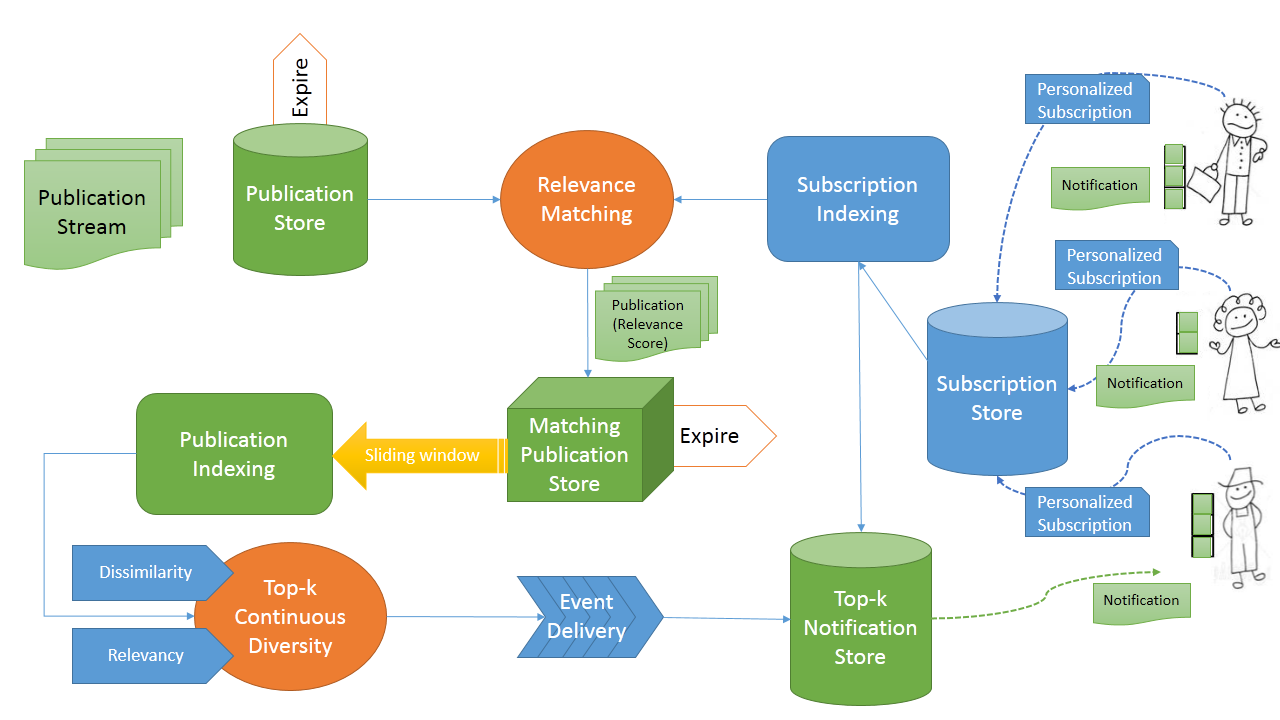
\includegraphics[scale=0.5]{images/Design_V1.png}
\caption{Top-k publish/subscribe architecture}
\label{our_pub_sub_architecture}
\end{center}
\end{figure}

In our design, we consider content-based publish/subscribe systems which offer greater expressiveness to subscriptions than topic or channel based ones. Also many researches believe that topic based publish/subscribe models are specialized forms of content-based models. In behavior level, our proposed top-k publish/subscribe model can be specialized into traditional publish/subscribe models easily either based on topic or content. In the rest of our study, our top-k matching model depends on the actual content of notification.
\paragraph*{}    
At the core of our proposed architecture, is a dual-indexing mechanism to partition the space in both subscriptions \& publications. Additionally the spaces are dynamic in the way the subscriptions support a variety of attributes under a large volume of subscription and also with the velocity of publication stream. The two indexing mechanisms are complementary ones, rather than distinct. In addition, we propose a subscriber friendly scoring algorithm which is linked with above modules to measure the effectiveness of the system.  

Since top-k publications are delivered across the stream, we adopt the notion of sliding window to further maximize the diversity of delivered results continuously. The diversified results are incrementally computed over consequent windows with the service of a personalized scheme. The system accepts preferential subscriptions from users with an ordered publication stream along with the time. We increase the stateful nature of the system by providing persistence subscription store with a publication store which is expired gradually to keep the freshness of the delivered output. Since our system supports the overlapping of user subscriptions, we also maintain an active notification store which share the query results over the set of same interested users.

\paragraph*{}
In more generic level, the overall architecture consists an efficient indexing module which is there to process top-k queries continuously. Later we shows that our indexing mechanism acts as a efficient module to implement the proposed approximation algorithm to deal with \emph{continuous k-diversity} problem.

\section{Scoring Algorithm}
\label{sec:scoring_algo}
\paragraph*{}
In top-k publish/subscribe models, publications trigger subscriptions based on a scoring algorithm. Most of the previous work proposed a threshold or bound based schemes where a subscription will be triggered by a new publication, iff it scores more than top scored publications previously published for this specific subscription \cite{Shraer2013}. Here, we combine above view with our approach where to deliver a diverse set of publications which is get-scored by query dependent metrics (e.g. Relevancy). Additionally the parameter k restricts the selection over the publication stream which is bounded by sliding windows along with the time. Diversified result set doesn't serve only top relevant elements but it also increases the freshness of them.


We have studied our problem in a restricted dynamic setting where the publications to be selected as top-k would change over time. Also subscriptions can be inserted or deleted but can not be changed once subscribed. Studying dynamic behavior of subscriptions is beyond our scope.

\subsection{Relevancy: Query personalization}
\label{sec:relevancy}
\paragraph*{}
Subscriptions are used to filter relevant information and also to disregard irrelevant information. So they're queried to select only publications which satisfy the subscriptions. In traditional content-based approaches, users can only express their interest over a set of predicates or expressions in the subscription. But there, all subscriptions are considered equally. 
\subparagraph*{}
Here we brought our view to provide Top-k matching publications against a user subscription space which user is subscribed into. We avoid using the traditional approach on keeping user subscriptions independently, which is tailor made for Boolean publish/subscribe matching models, but not for Top-k matching.

\subsubsection{Discussion}
\paragraph*{}
Any user may subscribe into many overlapping subscriptions independently in traditional model, where delivered publications on each subscription to a particular user will have many duplicate results. In recent literature, there are two most common techniques to reduce this overhead, \emph{subscription covering} \& \emph{subscription merging} \cite{Pripuzic2010}.

\begin{figure}[h]
\begin{center}
\includegraphics[scale=0.5]{images/sub_pref_v1.png}
\caption{Subscription covering vs. Subscription Merging vs. Attribute Merging}
\label{sub_pref}
\end{center}
\end{figure}

\paragraph*{Subscription Covering}
\begin{definition}[Subscription Covering]
A Boolean subscription is covered by another Boolean subscription if every publication which matches the former subscription also matches the latter subscription.
\end{definition}

\subparagraph*{Remarks}
\begin{itemize}
\item Subscription $s_1$ is covered by subscription $s_2$ does not imply that the subscription $s_1$ covers the subscription $s_2$. Thus, subscription covering is non-commutative [Figure \ref{sub_pref}.a].
\item Deciding whether a Boolean subscription is covered by a set of previously defined subscriptions was proven to be co-NP complete \cite{Pripuzic2010}
\item There is a high probability on adding redundant subscriptions. Thus, if a new subscription is already covered by the existing subscriptions, adding former is useless.
\item Reduce the flexibility of dynamic subscriptions, when the subscriber remove all subscriptions that are covered by another subscription, the latter becomes uncovered, and the opposite. So the validity of defined relation between subscriptions, should be updated more often.
\end{itemize}

\subparagraph*{Subscription Merging}
\paragraph*{}
Subscription merging is a specialized form of subscription covering. [Figure \ref{sub_pref}.b]
\begin{definition}[Subscription Merging]
Two or more Boolean subscriptions can be merged together in a broader subscription which then covers all of the original subscriptions.
\end{definition}

\paragraph*{Remarks}
\begin{itemize}
\item Boolean subscriptions can be merged together in perfect or imperfect way. In perfect merging, any part of the resulting subscription is covered by original subscription, but in imperfect merging it may not.
\item Imperfectly merged subscription may effect on the accuracy of matching publications as they can fall into any sub-interest of space which is not covered by the original subscription.
\end{itemize}

\paragraph*{}
If we allow to cover subscriptions in our approach on delivering Top-k results, we would have defined a way to cover the relation between preferences among subscription tuples and, the parameter $k$ which is dependent on the given subscription. Along with the identified complexity over boolean subscription covering, we can observe that former approach won't provide any benefit in top-k subscriptions but avoiding rare cases. Even though we reduce the subscription space, it may incur additional complexity level to our system. Subscription merging is also questionable under above scenario as it was a specialized case of subscription covering.
%Top-k subscriptions offer more representative power than boolean subscriptions. If we look at our personalized subscriptions, we allow the user to make preferences among attributes as well as to change the parameter $k$ to restrict the incoming publications. Additionally it may explicitly or implicitly change the neighborhood $\alpha$ which is offered by any publication. 
%
%If we allow to cover subscriptions in our approach, we would have defined a way to cover the relation between attribute preferences, $k$ and $\alpha$ also. With the identified complexity over boolean subscription covering, we can observe that former approach won't be useful in top-k subscriptions by avoiding rare cases. Even though we reduce the subscription space, it may incur additional complexity level to our system. Subscription merging is also questionable under above scenario.

\subsubsection{Proposed Model: Relating Attributes}
\label{sec:relatingatt}
\paragraph*{}
In top-k publish/subscribe models, it's preferred to have a degree of user interest over subscription space either locally or globally [Figure \ref{subscriber_preference_models}]. Many research works did consider to employ preferences among subscriptions \cite{Drosou2008, Drosou2009, Drosou2009workshopp}. Preference aware subscriptions can be used to rank the publications \& to deliver the user most preferred ones. In this way, preferences can be defined among subscriptions globally or among attributes in the particular subscription locally. Both qualitative \& quantitative approaches to compare attributes or subscriptions have been tried out \cite{Drosou2009workshopp}. But still user has to explicitly define the ordering between them.

\paragraph*{}
In our model, we try to represent more relations between subscription tuples to increase the representative power of user in the personalized subscription space. The relation between those tuples is presented by a directed graph where nodes represent subscription tuples \& the edges represent the relative preferences. The graph is dynamically changing it's behavior based on user intent. 

Subscribers can specify the degree of interest over the subscription space by defining a relative preference score on each subscription tuples which he subscribe into. From that local ordering of subscription tuples, the model can define a global ordering in the subscription space which is aggregated by above tuples. Each ordering is specifically defined for every subscribers. We consider user subscription spaces rather than each subscriptions independently. So we're not restricted on particular \ac{DNF} or \ac{CNF} to define the subscription, but on enhancing more user representative power in our model.

\begin{figure}[h]
\begin{center}
\includegraphics[scale=0.5]{images/pref1.png}
\caption{Subscriber preference models}
\label{subscriber_preference_models}
\end{center}
\end{figure}

\subparagraph*{}
A publication is scored against a satisfied subscription subspace instead just matching a publication whenever there is a satisfied subscription like in traditional models. In this way, our model can support partial matching between publications \& subscriptions, but still can provide top-k results. Overall, our approach is subscriber friendly where publications are ranked by the relation of subscriptions. We don't consider to make explicit publisher preferences on publications independently as it may destroy our research goal.



\begin{example}[\label{ex:subs}]
Let's assume that, Bob would like to get notify on products related with following personalized queries:
\begin{center}
$Q_1=\{carrier=AT\&T(0.4)\ \vee brand=HTC(0.3)\ \vee storage\leq16GB(0.7)\}$
$Q_2=\{carrier=Verizon(0.5)\ \vee storage\leq32GB(0.2)\}$
$Q_2=\{brand=HTC(0.3)\ \vee storage\leq32GB(0.6)\}$
\end{center}
using our top-k pub/sub model. If we represent them in our preference graph [Figure \ref{pref_graph}]

\begin{figure}[h]
\centering
    \subfloat[Constructing attribute preference graph]{{\includegraphics[scale=0.35]{images/sub_pref1.png} }}
    \qquad
    \subfloat[Attribute preference graph]{{\includegraphics[scale=0.35]{images/sub_pref2.png} }}
    \caption{Preference graph on $Q_1,\ Q_2,\ Q_3$}
    \label{pref_graph}%
\end{figure}

\subparagraph*{}
A seller publishes a product 
\begin{center}
$P_i=\{carrier=AT\&T\ \vee brand=HTC\ \vee storage\leq32GB\ \vee color=Black\ \vee OS=Android\} $
\end{center}
to our matching model. then the satisfying subspace of interest over user subscription space is: [Figure \ref{pref_graph2}]

\begin{figure}[h]
\begin{center}
\includegraphics[scale=0.5]{images/sub_pref3.png}
\caption{Satisfying subscription space}
\label{pref_graph2}
\end{center}
\end{figure}

Now, from our relevancy score function $r(p_i,\ Bob)$ we can calculate the relevancy score of product $p_i$. Then we can proceed with the next phase of our model to see whether the product will be selected as one of top-k products which are delivered to Bob eventually.
\end{example}

\subsubsection{Relevancy score}
\paragraph*{}
Relevance score of a publication can be computed as average sum of degree of interest $r(p_i)$ in preference relations where a higher score implies that the publication is more relevant. Note that, we don't consider certain degree of interest on corresponding tuples of subscriptions to calculate the score. Instead, we allow a finer granularity by taking the weighted relation between tuple preferences to calculate personalized score.

\begin{figure}
\begin{center}
\includegraphics[scale=0.5]{images/pref2.png}
\caption{Local \& Global ordering of preferences}
\label{local_global_ordering}
\end{center}
\end{figure}

\begin{definition}
Let $S^X$ be the the space of user personalized subscriptions submitted by user $X$, assume the set $S^X_{p_i}$ be the subset of $S^X$; $S^X_{p_i} \subseteq S^X$ which is satisfied by the publication $p_i$ in stream of publications $P;\ \forall p_i \in P$, the relevancy score is;
\begin{center}
\[ r(p_i,X)= \frac{ \sum_{u,v\in p_i\ \cap \ u,v \in S^X_{p_i}} G(u,v,w)}{|E|} \]
\[ where\ G(u,v,w)\ is\ the\ personalized\ subscription\ graph\]
\[ s.t.\ the\ edge\ weight\ w(u,v)=\frac{pref(v)}{pref(u)};\ (u,v) \in G(u,v,w) \]
\end{center}

$r(p_i,X)$ depicts the personalized relevancy score of a publication $p_i$ for a particular subscriber $X$ by calculating the average edge weights of covered edges from the intersected tuples between a publication \& the covered user subscription space $u,v\in p_i\ \cap \ u,v \in S^X_{p_i}$.
\end{definition}

In the section \ref{sec:sub_indeing} we extended the functionality of an efficient in-memory index (i.e. opIndex \cite{Zhang2014}) to adopt the notion of above model to calculate publications' relevancy. That is also scalable to the volume and update of subscriptions, the arrival rate of events and the variety of subscribable attributes. All publications which satisfy $r(p_i)>0$ forward to the next phase of our model to get diversified.

\subsection{Events Novelty}
\paragraph*{}
Personalization become the most influence factor so far to retrieve top-k results, but we observe that older publications may prevent the newer publications to enter into top-k results. Here we show some pros \& cons on ways to compute top-k results under different time policies (i.e. continuous, periodic, sliding window).
%\section{Top-k Matching: When?}
%\paragraph*{}
%Our Top-k event notification service is centralized where we need to deal with particular time policy for the computation \& delivery of Top-k results. The times, when the top-k publications are computed by the system \& when the publications are delivered to relevant user can be independent. In this section, we analysis different timing policies to compute top-k results. 

\begin{itemize}
\item \textbf{Continuous:} We can compute top-k result set continuously when new publications arrive. When publications are constantly produced, older publications may prevent new ones from reaching the user. We can associate an expiration time with each publication in the way that valid publications are not expired ones. In this way, older publications which have expired do not prevent new ones from reaching the users. But here, the number of delivered publications may depend on the relative order between them.
\begin{example}
Take an incident where publications are produced in the ascending order of their ranks, then all will be delivered, but in reverse only a part of them will
\end{example}
\item \textbf{Periodic:} Time can be divided into chunks of periods T, and top-k publications can be computed in each period. We can embed an expiration time as before to overcome the problem in continuous top-k computation. But clearly the computation of top-k results are depended on the duration of the time period. Also the velocity of events could effect final result.
\begin{example} 
Take an incident, where higher-ranked publications may produce in a given period, then some of them may be dropped due to the competition. But when lower-ranked publications are produced constantly in the given period, they will be delivered irrespective to the future higher rank publications.
\end{example}

\item \textbf{Sliding Event-window} We can compute top-k results based on publications within a moving event window (Ex: within w publications) to overcome above problem in periodic delivery. Hence, we can experiment with dynamic windows (variant w) \& jumping windows (Ex: less than w-1 overlapping between consequent windows). We also use our relevancy decay function inside an event window to avoid the problem in continuous top-k computation. To deal with more general data streams, we consider sliding event windows instead of sliding time windows. [Figure \ref{sliding_window_approach}]
\end{itemize}

\subparagraph*{}
As a motivation, a popular news pub/sub system like Google news maintain publications within last 30 days, but most of the time produce top-k results within last day or two. This phenomena is not particular to Top-k pub/sub but for most \ac{DSPS} in general \cite{Cormode2009}. Most common approach is to apply a function of \emph{time decay} that is not new in temporal data analysis. It often uses based on different aging techniques in a wide range of data processing applications.

When dealing with continuous query processing systems, it's obvious to produce stream of results. There has been a great deal of work on algorithms for efficiently answering streaming queries under complex time decay algorithms. But most of the algorithms failed to be scalable within streaming systems under sliding widows \cite{Cormode2009}.

\paragraph*{}
There are different classes to measure the age of a publication. One straightforward class is to measure the age since the publication was born in the system. In this approach, age is calculated back from the current time. But when updating the scores of continuous incoming publications in the query processing windows, we have to refresh \& update the age of all relevant publications. Due to this high inefficiency, \cite{Cormode2009} proposed "forward age" of an item which is relative to a landmark. The natural observation of above aging technique is that once it has been observed then it is fixed. 

\begin{definition}[General Decay Function]
Let $P$ be stream of publications where $(p_i, t_i)$ denotes a timestamped publication s.t. $ \forall (p_i, t_i) \in P$. We define the decay function $w(t_i, t)$ given at the current time $t$ \& $t_i$ be the publication time of $i^{th}$ publication, if it satisfies the following properties:
\begin{enumerate}[label=(\roman*]
\item $ \ w(t_i, t)=1\ when\ t_i=t,\ and\ 0\geq w(t_i, t) \leq 1;\ \forall t\geq t_i $
\item $ \ t' \geq t \rightarrow w(t_i, t')\leq w(t_i, t) $
\end{enumerate}

The definition says that relative decay score should always be $ 0 \geq w(t_i, t) \leq 1 $ for given time $t$, and it does not increase as time increases. So the decay score is always decreasing by providing the age of a publication can be called dead when it's decay score become $0$.
\end{definition}

\paragraph*{Forward Decay Function}
As the drawback which we identified earlier in \emph{backward decay} functions, here we rely on a \emph{forward decay} function. Let us define the general \emph{forward decay} function.

\begin{definition}[\label{def:fdecay}]
Given a positive monotone non-decreasing function $g$, and a landmark time $L$, the decayed score of a publication with arrival time $t_i > L$ which  measured at time $t \geq t_i$ is given by,
\begin{center}
\[ w(t_i, t)=\frac{g(t_i-L)}{g(t-L)} \]
\end{center}
Observe that, above decay function also satisfies the conditions hold by the general decay function.
\end{definition}

To decay time, the most natural choices of functions $g$ fall into different classes (i.e. no decay, polynomial decay, exponential decay, logarithmic decay, landmark window). Studying the relation between above classes is beyond our scope. We direct the reader to see \cite{Cormode2009} for further analysis.

\subsubsection{Discussion on selecting the right landmark}
\paragraph*{}
We can consider the smallest time-stamp of the publication stream as our landmark $L$, so all other publications are scored relative to it. But it's impossible to have a general view of the incoming publication stream at given time $t$. Even we're aligned with sliding windows, it may lead to compute decay score in every window. Due to above inefficiency, we observe that the default for $L$ should be the time when the subscription was issued. Since we deal with satisfying subscriptions as whole space, but not with particular subscriptions individually, getting the issued time of one subscription as a single landmark could effect our approach. Without losing generality we take the earliest issued time of the subscription (lower bound) among the subscription space which is submitted by a particular user as our landmark time $L$. 
\subparagraph*{}
But the selection of any landmark, is dependent on the class of decay function $g$ which is being applied. As an example, take the class of exponential to apply the landmark time.

\begin{center}
\[ w(t_i, t)=\frac{g(t_i-L)}{g(t-L)} \]
\[ w(t_i, t)=\frac{exp( \delta (t_i-L))}{exp( \delta (t-L))}\]
\[  s.t. g(a)=exp(\delta.a)  \]
\[ w(t_i, t)= exp( \delta (t_i-t)) \]
\end{center}

We can observe that above \emph{forward decay} function does only rely on the creation time of the given publication, but not on a landmark of time. That leads us to rely on exponential decaying function as it avoids the overhead of maintaining temporal properties of subscriptions, and also the recalculation of relative scores. Because as time grows, relative ranking between incoming publication does not vary, since at any given time $t$, it is equal for all publications. 

\begin{center}
\[ w(t_i, t)= exp( \delta t_i) \]
\end{center}

\subsubsection{Decaying Relevancy}
\label{sec:decayrel}
\paragraph*{}
To attach decaying with the scoring algorithm, we use it as a multiplier of the relevance score of a publication.

\begin{definition}
Let $P$ be stream of publications where $(p_i, t_i)$ denotes a timestamped publication s.t. $ \forall (p_i, t_i) \in P$, and given the decay function $w(t_i, t)$ given at the current time $t$ \& relevancy scoring function $r(p_i,X)$ for the user X, decaying relevancy function is,
\[ r^t(p_i,\ t_i,\ X)=r(p_i,X).w(t_i, t)\]
The decaying relevancy function $r^t(p_i,\ t_i,\ X)$ depicts the relevancy of a publication which decays along with the time. 
\end{definition}


\paragraph*{Remark:} When a new publication arrives, we avoid updating the scores of all other publications within a sliding window since the relative ranking between them is fixed due to the forward decay function. When the window is moving forward, earlier publications are getting dropped due to temporal constraints.

\subsection{Events Diversity}
\paragraph*{}
Instead of achieving pure personalized relevant results, one can view to increase the diversity of results to increase user satisfaction. Because getting similar top-k results is a natural drawback in most personalized query engines. Usually this happens when the subscription doesn't express finer granularity. But getting diverse set of results is proved to be a necessary condition to be effective in most information processing engines. We believe that applying diversity in our proposed model can further enhance top-k results set by exploring a wider spectrum. Because we support partial matching between publications \& subscriptions to have a set of breadth results. Hence, we don't have strong distinguishability between finer \& coarse granularity in the subscription themselves. Instead, our model selects diverse set of results from the matching publications with whole user subscription space. In our model, we support diversity aware top-k queries which maximize the diversity of top-k result set.

Specially our setting can be applied to e-commerce environment, where the trend as an uncertainty factor becomes the influence to increase buying. When our model does provide maximal diversity, there's a high probability where the most of the delivered products' information can cover the whole trend product set too.     

As an example, Bob would like to get notify about smart-phones from the carrier=AT\&T and brand=HTC. Without the notion of diversity, delivered top-k publications may have much similarity between them. Even though, the received publications are personalized, Bob may recognize such a system as non-effective. 

\paragraph*{}
Most previous approaches to define diversity are based on:
\begin{enumerate*}[label=(\roman*)]
\item (Dis)similarity
\item Coverage
\item Novelty
\end{enumerate*}
\cite{Drosou2010DiversitySurvey}, but sometimes combining more than one of them \cite{Drosou2012,Drosou2010DiversitySurvey}. In the top-k publish/subscribe context, diversity based on dissimilarity (i.e. delivered publications are dissimilar to each other), coverage (i.e. delivered publications can cover many interpretation of subscribers' information needs) \& novelty (i.e. publications which are presented earlier has higher priority) are considered orthogonally in more general versions, but have not spoken the applicability of them dependent on the applications. We believe that the definition of diversity is application dependent. Selecting the right definition of diversity under e-commerce environment in top-k publish/subscribe environment is one of our research output. 

Generally, in any form of definition, the diversification problem has been shown to be NP-hard \cite{Drosou2009} and hence provide heuristics for its approximation. Our study is based on a specialized form of \textbf{k-diversity} problem which is aligned with \emph{continuity} requirements introduced by \cite{Drosou2014ExtendedDiversity} to deal with data-stream. Hence, we focus on \textbf{continuous k-diversity problem}.


\subsubsection{k-diversity problem}

\paragraph{Based on dissimilarity}

\begin{definition}[k-diversity problem]
Let $P$ be the set of matching publications; $|P| = n$, and given a distance metric $d$ to express the dissimilarity between publication points, finding the diverse set S\textsuperscript* of $P$ such that:
\begin{center}
\[ S^* = arg\ max\ f(S, d);\ S \subseteq P;\ |S| = k;\ k \geq 0 \]
\end{center}
To calculate the distance between two publication points Minkowski, Euclidean or Angular (e.g. cosine-similarity, BM25) distance functions are widely used based on the applicability.

Three widely used functions (f) to aggregate the distances are MIN (i.e. minimum distance among selected items), SUM (i.e. sum of the distance among selected items) \& AVG (i.e. average distance among selected items). 

\begin{center}
\[ f _{MIN} (S,d) = min\ d(p_{i}, p_{j});\]
\[ f _{AVG} (S,d) = \frac{2}{k(k-1)}\sum_{i=1}^{k}\sum_{j>i}^{k} d(p_{i}, p_{j});\]
\[ f _{SUM} (S,d) = \sum\ d(p_{i}, p_{j});\]
\[such\ that \ p_{i}, p_{j} \in S;\ p_{i} \neq p_{j} \]
\end{center}

Above functions are known as \emph{MAXMIN}, \emph{MAXAVG} \& \emph{MAXSUM} in k-diversity problem. MAXMIN does select S\textsuperscript*;$|S^*|=k;$ out of P given points, so that the minimum distance between any pair of chosen points is maximized \cite{Drosou2010DiversitySurvey}. Instead of minimum, MAXAVG selects S\textsuperscript*;$|S^*|=k;$ out of P given points, so that the average distance between any pair of chosen points is maximized. In the same manner, MAXSUM selects S\textsuperscript*;$|S^*|=k;$ out of P given points, so that the sum of distance between any pair of chosen points is maximized.

\paragraph*{}
The general problem for most of these criteria is NP-hard which is extensively studied as dispersion problem in the literature. Approximation algorithms have been developed \& studied. We direct the reader to see \cite{Chandra2001} for the summary of results.

\end{definition}

\paragraph{Based on coverage}
\begin{definition}
Let $P$ be the set of matching publications; $|P| = n$, given a query $q$, a taxonomy $C$ \& a probability distribution $P(\frac{c}{q})$ for each category $c \in C$ that is relevant to C, finding the diverse set S\textsuperscript* of $P$ such that:
\begin{center}
\[ S^* = arg\ max\ P(\frac{c}{q}) \]
\end{center}
With above view, at least one selected publication in $S^*$ may cover the query relevant category $c$, so it maximizes the probability of former covering.
\end{definition}

\begin{definition}
Let $P$ be the set of matching publications; $|P| = n$, given a neighborhood $N^+_r(p_i)$, finding the diverse set S\textsuperscript* of $P$ such that:
\begin{center}
\[ \forall p_i \in P, \exists p_j \in N^+_r(p_i),\ s.t.\ p_j \in S\
s.t.\   N^+_r(p_i) =  N_r(p_i) \cup \{ p_i \} \]
where the neighborhood $N_r(p_i)$ of an object $p_i \in P$ \\
\[ N_r(p_i) = \{p_i\ |\ p_i \neq p_j\ \wedge d(p_{i}, p_{j} \leq r\};\ r\geq0 \]
\end{center}
With above view, publications in the neighborhood $N^+_r(p_i)$ of $p_i$ are considered similar with $p_i$ \& covered by $p_i$.
\end{definition}

\paragraph{Based on novelty}
A precise distinction between novelty \& diversity has been made by \cite{Clarke2008} in the context of \ac{IR} systems. Novelty is used to resolve redundancy while diversity is to resolve ambiguity. In the context of top-k publish/subscribe, the notion of novelty is used separately from diversity where to avoid the blocking of delivered new publications by old publications.  

\paragraph{Proposed Model: MAX* k-diversity}
\paragraph*{}
Up to the treatment of diversity, any model has general top-k retrieval properties. By taking one of "off-the-shelf" diversity definitions won't guarantee to retrieve an effective result set in the context of top-k publish/subscribe. Many definitions are tailor made to problems in \ac{IR} \& database community. From the efficiency point of view in our proposed model, calculating diversified results over the stream may have a big part to reduce the processing cost of top-k matching. We believe that it's crucial to select the right definition to suit our problem domain.

In our study, we address diversity through a different perspective. Based on the explanation which is provided by the subscriber to retrieve top-k publications, we propose two diversification methods called as: (where $S^* \in P;\ |S^*|=k;\ |P|=n$)
\begin{enumerate}
\item MAXMINPSCORE: a combination of MAXMIN dissimilarity based on item distance as well as MAXSCORE to maximize the sum of relevance score on the selected k items. 
\item MAXMINNSCORE: a combination of MAXMIN dissimilarity based on item distance as well as MAXSCORE to maximize the negative sum of relevance score on the dropped n-k items.
\end{enumerate}

Our view on combining relevance with diversity is motivated by the natural axioms presented by \cite{Gollapudi2009}. 

\paragraph*{MAXMINPSCORE k-diversity problem}
\begin{definition}
Let $P$ be the set of matching publications; $|P| = n$, and given a distance metric $d$ to express the dissimilarity between publication points \& relevancy function $r$ to depict the relevance of a publication which is calculated according to the degree of user interest where $\lambda > 0$ is a parameter that tunes the importance of diversification, finding the diverse set S\textsuperscript* of $P$ such that:

\begin{center}
\[ S^* = arg\ max\ f(S,\ d,\ r);\ S \subseteq P;\ |S| = k;\ k \geq 0 \]
\[s.t.\ f(S,\ d,\ r)= ( \lambda.f(S, d)+(1-\lambda).f(S, r) )\]
\[where\ f _{MIN} (S,d) = min\ d(p_{i}, p_{j});\ and,\]
\[ f _{SCORE} (S,r) = \sum_{i=1}^{k}\ r(p_i);\]
\[such\ that \ p_{i}, p_{j} \in S;\ p_{i} \neq p_{j} \]
\end{center}
\end{definition}

We skipped the definition of MAXMINNSCORE k-diversity problem as it has the same logic instead of symbols.
\paragraph{Design philosophy}
But the proposed model can be re-casted in terms of a \emph{facility dispersion} problem, known as the MAXSUMDISPERSION problem \cite{Gollapudi2009}. We skip the proof for the time being, but we can map known heuristic based solutions to achieve our diversification objective as stated generally by \cite{Gollapudi2009}.
\subparagraph{Not to reinvent the wheel}
The design philosophy is not to re-invent the wheel by looking for new and novel techniques to implement heuristic based solutions for \emph{facility dispersion} problem. We have come up with another mono-objective formulation which does not relate with \emph{facility dispersion} as it combines relevance and diversity.

 
\paragraph{Beyond Diversity \& Relevance}
Instead of selecting the importance of the whole set $S^*$, now we select a set of diverse set which increase the "global" importance of a selected publication \& reduce the "global" importance of a non-selected publication. In the rest of our study, our definition of diversity will be called as MAXDIVREL.

\paragraph{MAXDIVREL k-diversity problem}
\begin{definition}
Let $P$ be the set of matching publications; $|P| = n$, and given a distance metric $d$ to express the dissimilarity between publication points \& relevancy metric $r$ to depict the relevance of a publication which is calculated according to the degree of user interest \& $\alpha$ is the neighborhood represented s.t. $d(p_i,\ p_j)\leq \alpha $, where $\lambda > 0$ is a parameter that tunes the importance of diversification, finding the diverse set S\textsuperscript* of $P$ such that:

\begin{center}
\[ S^* = arg\ max\ f_\alpha(S,\ d,\ r);\ S \subseteq P;\ |S| = k;\ k \geq 0;\ \alpha \geq 0 \]
\[s.t.\ f _\alpha(S,\ d,\ r) = \lambda.\ \frac{g _\alpha(S,\ d,\ r) \/ }{h _\alpha(S,\ d,\ r)} \]
\[where\ g _\alpha(S,\ d,\ r)=\frac{1}{|S|}.\sum_{p_i,\ p_j\in S} \frac{r(p_j)}{r(p_i)}.d(p_i,p_j)\ and,\]
\[h _\alpha(S,\ d,\ r)=\frac{1}{|P-S|}.\sum_{p_i\in S,\ p_j\in (P-S)} \frac{r(p_j)}{r(p_i)}.d(p_i,p_j);\ \]
\[such\ that \ p_{i} \neq p_{j} and\ d(p_i,\ p_j)\leq \alpha \]
\end{center}
\end{definition}

\paragraph*{}
Let us demonstrate the behavior of MAXDIVREL k-diversity problem. Let's assume that we can map the set of publications $P$ into 2-dimensional space. The relevancy score $r(p_i)$ is already assigned with each data-point where high scores are more important to user. Dissimilarity between two data-points can be calculated by any distance metric (e.g. Euclidean, Manhattan) from the 2-dimensional space. Two data points are considered as similar if they satisfy $d(p_i,\ p_j)\leq \alpha $, where $\alpha > 0$.

Now let's select the k MAXDIVREL diverse result set (red color points) by getting more relevant but dissimilar results while also reducing less relevant but similar results [Figure \ref{MAXDIVREL_demo}].


\begin{figure}[h]
\begin{center}
\includegraphics[scale=1]{images/poikilo1_v1.png}
\caption{MAXDIVREL demonstration using dummy data model}
\label{MAXDIVREL_demo}
\end{center}
\end{figure}


\subsubsection{Continuous k-diversity problem}
\paragraph*{}
As we're bounded by the sliding windows over the continuous data-stream, one could view to apply static version of diversity definition on each window \cite{Drosou2009Diversity,Drosou2012ExtendedDiversity}. But due to highly inefficiency of above straightforward solution, limited number of works \cite{Drosou2014ExtendedDiversity, Vee2008} have proposed incremental approximation algorithms to retrieve k diversified results on each window as continuous k-diversity problem is also known to be NP-Hard. 

\paragraph{Sliding window approach}
Since this is an instance of continuous data delivery, we need to address over which subsets we apply MAXDIVREL diversity. In recent top-k publish/subscribe literature, \emph{sliding window} concept has been emerged without the loss of generality of the publication stream \cite{Pripuzi2008, Drosou2009Diversity}.

In the rest of our study, we rely on forward sliding event windows as a time independent approach where items are only forwarded. This approach can be dynamically parametrized further by the event arrival rate. With sliding-window processing, the $k$ most diverse items are computed over sliding windows of length $w$ based on MAXDIVREL. 

\begin{figure}[h]
\begin{center}
\includegraphics[scale=1]{images/sliding_window.png}
\caption{Sliding window approach: $w = 5$}
\label{sliding_window_approach}
\end{center}
\end{figure}

If we again align with our design (Figure \ref{our_pub_sub_architecture}), we consider the case where the set of personalized relevant publications $P$ changes over time. That causes to update the previously computed top-k results effectively for each subscriber. 

\subparagraph*{}
When you focus on above computation more closely, you can have a observation that an addition of single publication to the set $P$ may result in a completely different set of diversified items in the worst case. Let us show to achieve the continuity requirements in continuous data delivery, above observation is crucial \& leads to have efficient incremental algorithms.

\paragraph{Continuity requirements} 
In continuous data delivery, we should have a set of requirements to achieve, that may depict the effectiveness of the system in the long run \cite{Drosou2014ExtendedDiversity}. 
\begin{enumerate}[label=(\roman*)]
\item \textbf{Durability}: We need to avoid uncertainty of appearing of diversified items on each window. Thus, an item is selected as diversified in $i^{th}$ window may still have the chance to be in $(i+1)^{th}$ window if it's not expired \& other valid items in $(i+1)^{th}$ window are failed to compete with it.
\item \textbf{Order} The order on how we compute the set of top-k items will follow the chronological order. When the matching publications are timestamped, we avoid the selection of item $j$ as diverse later, when we already selected an item $i$ which is not-older than $j$. To consider cause-effect order \& other complex relations among publications is beyond our scope.
\end{enumerate}

\paragraph{MAXDIVREL continuous k-diversity problem}
\label{MAXIVREL_condiv}
\begin{definition}
Let $P=\{P_i,P_{i-1},...,P_1\}$ be a stream of set of publications over sliding windows $w=\{w_i,w_{i-1},...,w_1\}$, be
any two consequent windows $w_{i-1},w_i$ and $S^∗_{i−1}$ be the diverse subset of $P_{i-1}$, selecting the subset $S^*_i$ of $P_i$ at window $w_i$  such that satisfying MAXDIVREL k-diversity problem at each instance,
\begin{center}
\[ S^*_i = arg\ max\ f_\alpha(S_i,\ d,\ r);\ S_i \subseteq P_i;\ |S_i| = k;\ k \geq 0;\ \alpha \geq 0 \]
\[s.t.\ f _\alpha(S_i,\ d,\ r) = \lambda.\ \frac{g _\alpha(S_i,\ d,\ r) \/ }{h _\alpha(S_i,\ d,\ r)} \]
\[where\ g _\alpha(S_i,\ d,\ r)=\frac{1}{|S_i|}.\sum_{p_i,\ p_j\in S_i} \frac{r(p_j)}{r(p_i)}.d(p_i,p_j)\ and,\]
\[h _\alpha(S_i,\ d,\ r)=\frac{1}{|P_i-S_i|}.\sum_{p_i\in S_i,\ p_j\in (P_i-S_i)} \frac{r(p_j)}{r(p_i)}.d(p_i,p_j);\ \]
\[such\ that \ p_{i} \neq p_{j} and\ d(p_i,\ p_j)\leq \alpha \]
\end{center}
where it must satisfies the continuity conditions hold by \emph{durability} \& \emph{ordering}.
\end{definition}

We show that top-k MAXDIVREL query is NP-hard and propose a greedy heuristic based technique to compute an approximation of the optimal answer set.

\subparagraph{Uniqueness}
Our approach is different than previous top-k bounded diversification methods which rely on associating a diversity score with each object in the result and then either selecting the top-k highest ranked objects or those objects whose score is above some threshold. We're motivated by most recent works \cite{Drosou2012, Qin2012, Ranu2014a} to diversify top-k results based on a neighborhood based method. But overall our approach does concern under a dynamic setting where the subscription \& publication space may change frequently which in results need to update computed top-k results. Also we do concern to maximize the representative power of the top-k results by considering both selected $(S)$ \& non-selected $(P-S)$ sets.

%\subparagraph*{DisC diversity \cite{Drosou2012}}

%\subparagraph*{Diversifying Top-k results \cite{Qin2012}}

%\subparagraph*{Top-k Representative Queries on graph databases \cite{Ranu2014}}

\subparagraph{Properties}
As general diversification problem is NP-Hard, we analyze the complexity of MAXDIVREL. We can show that MAXDIVREL can be reduced into Top-k representative query problem in graph databases where it's proved to be NP-Hard \cite{Ranu2014a}. For the time being, we omit the proof. But we show a simple greedy approach which is an extended version of general k-diversity problem [Algorithm \ref{Greedy_MAXDIVREL}]. 

\begin{algorithm} 
  \caption{Greedy MAXDIVREL: Extended version of Greedy-DisC}
  \label{Greedy_MAXDIVREL} 
  \algorithmicrequire \ Initial set of publications $P_r$ with $k$ wanted publications,\\ and the neighborhood threshold $\alpha$ \\
  \algorithmicensure \ MAXDIVREL subset of $S;\|S|=k$
  \begin{algorithmic}    
    \State compute $P_r$
    \State $S \leftarrow \phi$
    \For  {$\forall p_i \in P_r$} 
    \State color $p_i$ white
    \EndFor
    \While {$\exists \ white\ p_i \in P_r$ }
    \State select white $p_i$ with the largest $MAXDIVREL_{p_i}$
    \State $S \leftarrow S \cup {p_i}$
    \State color $p_i$ black
    \For  {$\forall p_j \in P_r \cap N_\alpha(p_j)$} 
    \State color $p_j$ grey
    \EndFor
    \EndWhile
    \State return $S$    
  \end{algorithmic} 
\end{algorithm} 

But in the streaming windows, calculating incremental neighborhood is seemed to be the place having performance bottleneck. We further analyze our basic greedy approach to suit into sliding windows \& experiment with index based mechanism to provide incremental MAXDIVREL algorithm. We show our index based approach in section \ref{sec:pub_index}.

\section{Explore Subscription parameters}
\label{sec:sub_param}

\section{Events Delivery}
\label{sec:delivery}
\begin{figure}[H]
\begin{center}
\includegraphics[scale=0.75]{images/Event_notification_v1.png}
\caption{Centralized Top-k publish/subscribe architecture}
\label{img:centralized_pub_sub}
\end{center}
\end{figure}

\paragraph*{}
The architecture of our top-k publish/subscribe system is a client-server architecture in which all subscribers \& publishers are connected to a centralized cloud based publish/subscribe service (Figure \ref{img:centralized_pub_sub}). Event delivery can be done pro-actively (within static or dynamic time units) or on-demand. But building efficient routing strategies for top-k matching \& delivery is beyond our scope.
 
\chapter{Indexing}
\paragraph*{}
In this chapter, we show our dual-indexing mechanism in both subscription \& publication spaces. We analyze different space-cutting data structures which are more efficient to suit into our design \& architecture.

\section{Subscription Indexing}
\label{sec:sub_index}
\paragraph*{}
In our model, we consider subscription spaces per user which express a specific user interest over the global subscription space by all users. But computing the relevancy function over large subscription space may increase the processing time of top-k results. Note that, our mechanism should be scalable under variety of attributes to deal with natural phenomena in e-commerce domain.
\subparagraph*{}
In traditional publish/subscribe models, we need to locate at least one subscription, for matching to be completed successfully. Recent literature in publish/subscribe, proposed many indexing structures which addressed above scenario of locating relevant subscription. But here we need to locate all matching subscription tuples in the space to compute the relevancy of a publication. So we adopt novel index method called OpIndex \cite{Zhang2014} which was introduced in state-of-the-art publish/subscribe to extend it's functionalities to suit with our preference relation model. 

\subsection{OpIndex}
\paragraph*{}
OpIndex organizes the subscription predicates into disjoint subsets each of which is independently and efficiently indexed to minimize the number of candidate subscriptions accessed for event matching. Also it outperforms other competing index based methods(e.g. k-index, BE-Tree) based on performance metrics like index construction time,memory cost and query processing time. OpIndex is built over inverted-list: a data-structure which is extensively studied over decades. Additionally, space cutting techniques (i.e. two level partition scheme) used at OpIndex, is specifically built to handle \emph{variety} of data that is natural under e-commerce along with the \emph{volume} of subscriptions \& high \emph{velocity} of publications. As most other pub/sub indexing mechanisms can't cope effectively on the variety of data, we believe OpIndex is the right choice by it's evaluation which was done using comprehensive space \& time complexity analysis.
\subparagraph*{}
In the first level, OpIndex select a pivot attribute by modeling it as visibility minimization problem \cite{Zhang2014} for each subscription, and subscriptions with the same pivot attribute are grouped together. In the second level, subscriptions are further partitioned based on their predicate operators. 

\paragraph*{Level 1: Attribute partitioning}
Here, we demonstrate level 1 partitioning based on subscriptions presented at table \ref{ta:exsub} which are commonly used at traditional publish/subscribe models.

\begin{table}[ht]
\caption{Example subscriptions} % title of Table
\centering % used for centering table
\begin{tabular}{c c} % centered columns (4 columns)
\hline\hline %inserts double horizontal lines
ID & Subscription \\ [0.5ex] % inserts table 
%heading
\hline % inserts single horizontal line
$S_1$ & $carrier=AT\&T\ \wedge brand=HTC\ \wedge storage\leq16GB$ \\ % inserting body of the table
$S_2$ & $carrier=Verizon\ \wedge storage\geq32GB$ \\
$S_3$ & $brand=HTC\ \wedge price\leq\$300$ \\ [1ex] % [1ex] adds vertical space
\hline %inserts single line
\end{tabular}
\label{ta:exsub}
\end{table}

OpIndex uses \emph{pivot} attributes to partition the subscriptions into independent posting lists. To select a pivot attribute per subscription, OpIndex uses following proved lemma \ref{lemma:pivot}.   

\begin{lemma}[Pivot Attribute selection \label{lemma:pivot}]
Given a stream of publications E, using $\delta_S=arg_{A\in S}min \bigtriangleup(A)$ to select pivot attributes for partitioning subscriptions minimizes the number of candidate matching subscriptions accessed to match the events in E
\end{lemma}

$\bigtriangleup(A)$ denotes the frequency of an attribute $A$ in an event stream $E$. OpIndex choose attribute $A$ to be the pivot attribute for a subscription $S$ if $A$ appears the least frequently in $E$ among all the attributes in $S$.

\subparagraph*{}
Let $carrier$ \& $brand$ be the pivot attributes for the subscription (Table \ref{ta:subl1}). Then, we have two posting lists as depicted in Figure \ref{img:l1part}


\begin{table}[ht]
\caption{First level partitioning of subscriptions} % title of Table
\centering % used for centering table
\begin{tabular}{c c} % centered columns (4 columns)
\hline
Subscription & Pivot Attribute \\ [0.5ex] % inserts table 
%heading
\hline % inserts single horizontal line
$S_1$ & $carrier$ \\ % inserting body of the table
$S_2$ & $carrier$ \\
$S_3$ & $brand$ \\ [1ex] % [1ex] adds vertical space
\hline %inserts single line
\end{tabular}
\label{ta:subl1}
\end{table}

\begin{figure}
\caption{Attribute Lists}
\centering
\begin{tikzpicture}
\node [circle, draw] (a) at (0,0) {$L_{carrier}$};
\node [rectangle, draw] (b) [right=of a] {$S_1$};
\node [rectangle, draw] (c) [right=of b] {$S_2$};
\draw [-] (a) to (b);
\draw [-] (b) to (c);

\node [circle, draw] (a) at (0,-2) {$L_{brand}$};
\node [rectangle, draw] (b) [right=of a] {$S_3$};
\draw [-] (a) to (b);
\end{tikzpicture}
\label{img:l1part}
\end{figure}


\paragraph*{Level 2: Operator partitioning}
Each attribute(posting) list ($L_{(\delta_S)}$) is organized as an inverted-list structure based on the predicate operator into operator lists ($L_{(\delta_{(S,f_{op})})}$). Operator lists are sorted by the attribute and ties are broken by the comparison of value. Given on the operator in the publication tuples we can perform equality or range searches to locate the relevant subscription in the operating list.(Figure \ref{img:l2part}) They also used some optimizations techniques to speed-up range scans.

\begin{figure}[H]
\caption{Operator Lists on $L_{carrier}$}
\centering
\begin{tikzpicture}
\node [circle, draw] (a) at (0,0) {$L_{carrier}$};
\node [circle, draw] (b1) [above right=of a] {$=$};
\node [circle, draw] (b2) [right=of a] {$\leq$};
\node [circle, draw] (b3) [below right=of a] {$\geq$};
\node [rectangle, draw, fill=black!20] (c) [right=of b1] {$carrier=AT\&T$};
\node [rectangle, draw, fill=blue!20] (f) [right=of c] {$carrier=Verizon$};
\node [rectangle, draw, fill=black!20] (d) [right=of f] {$brand=HTC$};
\node [rectangle, draw, fill=black!20] (e) [right=of b2] {$storage\leq16GB$};
\node [rectangle, draw, fill=blue!20] (g) [right=of b3] {$storage\geq32GB$};
\draw [-] (a) to (b1);
\draw [-] (a) to (b2);
\draw [-] (a) to (b3);
\draw [-] (b1) to (c);
\draw [-] (c) to (f);
\draw [-] (f) to (d);
\draw [-] (b2) to (e);
\draw [-] (b3) to (g);
\end{tikzpicture}
\label{img:l2part}
\end{figure}

\subsection{Modified OpIndex}
\paragraph*{}
From OpIndex, we adopt only the concept of two level partitioning using inverted-lists. Because OpIndex was designed to deal with Boolean publish/subscribe model. Hence, it's capable enough to locate at least one matching subscription when a publication arrives. But as we described at section \ref{sec:comparisonbtop}, we don't rely on individual subscriptions. So we need to partition each subscription tuples and, relate the inverted-list of predicates based on user given preference. Instead of a set of inverted-lists, our model generates a weighted inverted-graph for each user subscription space.

\subparagraph*{}
Here, we demonstrate the two-level partition scheme we proposed on personalized subscriptions at Table \ref{table:pnonlin}
\begin{table}[ht]
\caption{Example personalized subscriptions} % title of Table
\centering % used for centering table
\begin{tabular}{c c} % centered columns (4 columns)
\hline\hline %inserts double horizontal lines
ID & Subscription \\ [0.5ex] % inserts table 
%heading
\hline % inserts single horizontal line
$S_1$ & $carrier=AT\&T(0.4)\ \vee brand=HTC(0.3)\ \vee storage\leq16GB(0.7)$ \\ % inserting body of the table
$S_2$ & $carrier=Verizon(0.5)\ \vee storage\geq32GB(0.2)$ \\
$S_3$ & $brand=HTC(0.3)\ \vee price\leq \$300(0.6)$ \\ [1ex] % [1ex] adds vertical space
\hline %inserts single line
\end{tabular}
\label{table:pnonlin} % is used to refer this table in the text
\end{table}

Since we're not restricted to keep the subscription itself, we don't need to use any pivot attribute to partition subscription tuples at the initial level. Instead every unique attribute in the subscription tuples are used to partition the space. It's been motivated by following natural observation presented at e-commerce domain \footnote{http://storecoach.com/ecommerce-glossary/attribute/}:

\begin{itemize}[label=$-$]
\item In a given user subscription tuple space, the number of unique attributes is less than the number of unique operands or values that are assigned to.
\begin{example}
Attributes (A)=$\{carrier,\ brand,\ storage,\ price\}$ where $|A|=4;$
Values (V)=$\{AT\&T,\ HTC,\ 16GB,\ Verizon,\ 32GB,\ \$300\}$ where $|V|=6$
such that $|A| \leq |V|;$
\end{example}
\end{itemize}

In the second phase of partitioning, available operators within the attribute lists are used to repeat the partitioning as earlier. (Figure \ref{img:mlpart})

\subsubsection{Index construction}
\begin{algorithm}
\caption{To be continued: Insertion \& update algorithms}
  \label{algo:indexinsert}
To be continued: Insertion \& update algorithms.....
\end{algorithm}


\begin{figure}[H]
\caption{Inverted-list two-level partitioning on user subscription space}
\centering
\begin{tikzpicture}
\node [circle, draw] (a) at (0,0) {$L_{carrier}$};
\node [circle, draw] (a1) [right=of a] {$=$};
\node [rectangle, draw] (a11) [right=of a1] {$carrier=AT\&T$};
\node [rectangle, draw] (a12) [right=of a11] {$carrier=Verizon$};

\node [circle, draw] (b) at (0,-2) {$L_{brand}$};
\node [circle, draw] (b1) [right=of b] {$=$};
\node [rectangle, draw] (b11) [right=of b1] {$brand=HTC$};

\node [circle, draw] (c) at (0,-6) {$L_{storage}$};
\node [circle, draw] (c1) [above right=of c] {$\leq$};
\node [circle, draw] (c2) [below right=of c] {$\geq$};
\node [rectangle, draw] (c11) [right=of c1] {$storage\leq16GB$};
\node [rectangle, draw] (c21) [right=of c2] {$storage\geq32GB$};

\node [circle, draw] (d) at (0,-10) {$L_{price}$};
\node [circle, draw] (d1) [right=of d] {$\leq$};
\node [rectangle, draw] (d11) [right=of d1] {$price\leq\$300$};

\draw [-] (a) to (a1);
\draw [-] (a1) to (a11);
\draw [-] (a11) to (a12);

\draw [-] (b) to (b1);
\draw [-] (b1) to (b11);

\draw [-] (c) to (c1);
\draw [-] (c) to (c2);
\draw [-] (c1) to (c11);
\draw [-] (c2) to (c21);

\draw [-] (d) to (d1);
\draw [-] (d1) to (d11);
\end{tikzpicture}
\label{img:mlpart}
\end{figure}


\subsubsection{Matching}
\paragraph*{}
Note that our goal is to maximize the representative power of user subscription space, to increase the importance of a matching publication. Since we have the structural view of our user subscription space, now we can derive the relation graph by assigning relative user preference scores as weights to align with our personalized subscription graph definition \ref{def:persubgraph} and, also described at section \ref{sec:relatingatt}.

Figure \ref{img:mlppart} depicts the personalized OpIndex that is demonstrated using preference values at Table \ref{table:pnonlin}. 

\begin{figure}[H]
\caption{Inverted-graph on personalized user subscription space}
\centering
\begin{tikzpicture}
\node [circle, draw] (a) at (0,0) {$L_{carrier}$};
\node [circle, draw] (a1) [right=of a] {$=$};
\node [rectangle, draw, fill=blue!20] (a11) [right=of a1] {$carrier=AT\&T$};
\node [rectangle, draw, fill=blue!20] (a12) [right=of a11] {$carrier=Verizon$};

\node [circle, draw] (b) at (0,-2) {$L_{brand}$};
\node [circle, draw] (b1) [right=of b] {$=$};
\node [rectangle, draw, fill=blue!20] (b11) [right=of b1] {$brand=HTC$};

\node [circle, draw] (c) at (0,-6) {$L_{storage}$};
\node [circle, draw] (c1) [above right=of c] {$\leq$};
\node [circle, draw] (c2) [below right=of c] {$\geq$};
\node [rectangle, draw, fill=blue!20] (c11) [right=of c1] {$storage\leq16GB$};
\node [rectangle, draw, fill=blue!20] (c21) [right=of c2] {$storage\geq32GB$};

\node [circle, draw] (d) at (0,-10) {$L_{price}$};
\node [circle, draw] (d1) [right=of d] {$\leq$};
\node [rectangle, draw, fill=blue!20] (d11) [right=of d1] {$price\leq\$300$};

\draw [-] (a) to (a1);
\draw [-] (a1) to (a11);
\draw [-] (a11) to (a12);

\draw [-] (b) to (b1);
\draw [-] (b1) to (b11);

\draw [-] (c) to (c1);
\draw [-] (c) to (c2);
\draw [-] (c1) to (c11);
\draw [-] (c2) to (c21);

\draw [-] (d) to (d1);
\draw [-] (d1) to (d11);

\draw [->] (b11) to node [auto] {$1.3$} (a11);
\draw [->] (a11) to [bend left=60] node [auto] {$1.75$} (c11);
\draw [->] (b11) to node [auto] {$2.3$} (c11);
\draw [->] (c21) to [bend right=45] node [auto] {$2.5$} (a12);
\draw [->] (b11) to [bend left=60] node [auto] {$2$} (d11);
\end{tikzpicture}
\label{img:mlppart}
\end{figure}

\begin{algorithm}
\caption{To be continued: Matching algorithm}
  \label{algo:indexmatch}
To be continued: Matching algorithm.....
\end{algorithm}

\section{Publication Indexing}
\label{sec:pub_index}
\subsubsection{Decide Top-k}
Recall that, publications are not static in the space, where they do follow an incoming stream. Publication stream is partitioned based on sliding windows. Hence, our goal is to avoid re-computation of Top-k publications at each window, but to incrementally add new "winning" publications at window $w$ to a portion of Top-k results at window $w-1$.

\begin{example}{Assumptic normal Top-k matching}
\label{ex:asscase}
\paragraph*{}
Let's take $w=5$ item based sliding window. We showed earlier how we compute Top-k($k=2$) results as publications $(P_1,P_2,P_3,P_4,P_5)$ within the window $w-1$ are indexed batch-wise. Now the decision has to be made on the next window $w$. (Figure \ref{img:incsw1})

As there are $w-1$ overlaps of publications between windows, the decision may be upon the newly added publication $P_6$ whether it can belong into the current Top-k or not. Then the problem arises when it belongs, to decide the $i^{th}$ publication to be replaced; $0 \geq i \geq k$
\end{example}

\begin{figure}[h]
\begin{center}
\includegraphics[scale=1]{images/swlsh.png}
\caption{Simple Top-k matching on sliding window approach: $w = 5$}
\label{img:incsw1}
\end{center}
\end{figure}

\paragraph{Discussion}
Maintaining Top-k results over incoming stream is dependent on the matching algorithm we're dealt with. As an example if Top-k matching happens based on a relevancy threshold, we can limit the problem scenario to the previous example \ref{ex:asscase}. But as we addressed in our problem statement, to deliver most diversified set of results based on MAXDIVREL, we can not rely only on the previously computed Top-k. This problem was identified at previous diversity algorithms (e.g. MAXMIN, MAXSUM, DisC) as well, but left alone by simply re-computing Top-k again.(Figure \ref{img:incsw2})

\begin{figure}[h]
\begin{center}
\includegraphics[scale=1]{images/swlsh2.png}
\caption{MAXDIVREL Top-k matching on sliding window approach: $w = 5$}
\label{img:incsw2}
\end{center}
\end{figure}

To decide Top-k at window $w$, we avoid re-computation of all previously seen publications at window $w-1$, but only compute newly added publications against most similar ones. This phenomena is motivated by the problem definition of MAXDIVREL diversity. Hence, our proposed indexing mechanism is urged by this particular problem.

\paragraph*{}
As we discussed in section \ref{MAXIVREL_condiv}, MAXDIVREL continuous k-diversity problem has a performance bottleneck when calculating neighbors in consequent sliding windows. To develop an incremental diversity algorithms based on similarity neighborhood, we can rely on a space-cutting data structure to select neighbors of a publication $p_i$ in the current window from the neighbor selection in the previous window. That may lead to index publications in each sliding window to compute dynamic top-k results in the long run. As we described at section \ref{sec:rwpubindex}, a couple of recent works on results diversification in database community adopt tree-based techniques to model their diversity problem \cite{Drosou2014ExtendedDiversity,Rao2012}

\subsubsection{Near Neighbor query}
Here, we try to align MAXDIVREL continuous k-diversity problem with \acf{NN} queries. \ac{NN} queries are extensively studied in static database community over different data-structures. 

\paragraph*{\acf{NN} query}
We say that a point $p$ is an $R-near\ neighbor$ of a point $q$ if the distance between $p$ and $q$ is at most $R$ (Figure \ref{img:rnn}).

\begin{figure}[h]
\begin{center}
\includegraphics[scale=0.75]{images/NN_Query.png}
\caption{$R$ near-neighbor query}
\label{img:rnn}
\end{center}
\end{figure}

%\paragraph*{\acf{NearestN} query}
%The nearest neighbor problem is an example of an optimization problem: the goal is to find a point which minimizes a certain objective function (in this case, the distance to the query point), Here we discuss only the decision version of \acf{NearestN}. It's important to observe that \ac{NearestN} problem also solves the R-\ac{NN} problem too.

\paragraph*{}
In our study, we focus on the approximate \acf{NN} problem. The formal definition of the approximate version of the \ac{NN} problem is as follows \cite{Indyk2008}:
\begin{definition}[Randomized c-approximate R-near neighbor]
Given a set $P$ of points in a $n$-dimensional space $\mathbb{R}^n$, and parameters $R > 0,\ \delta > 0$, construct a data structure such that, given
any query point $q$, if there exists an $R$-near neighbor of $q$ in $P$, it reports some $cR$-near neighbor of $q$ in $P$ with probability $1 - \delta$
\end{definition}

We rely on above definition, where in our case, we need to find $k$ query points that report $cR$-near neighbors at the probability of $1 - \delta^k$. Not depending on a linear search over high dimensional space that contain large number objects, existing data-structures to tackle above problem are trees, grid and hashes.

Due to most hierarchical models (range trees, kd-trees, B-trees, cover trees) don’t work well in high dimensions and, grid solutions (voronoi grid) are not accurate on boundary values, we will explore a technique called \acf{LSH} to find approximate (near) matches efficiently. LSH-based methods appear most effective when the degree of similarity we accept is relatively low. As we need to find points that have maximal dissimilarity on given publication space as Top-k results, we believe LSH is the most optimal data structure to adopt. 

A well-designed hash table allows a symbol lookup in $O(1)$ time with $O(N)$ memory, where $N$ is the number of entries in the table, and separates two symbols that are close together into different buckets. To find approximate (near) matches efficiently we use a locality-sensitive hash.

\subsection{Locality Sensitive Hashing (LSH)}
\label{sec:lsh}
\paragraph*{}
\ac{LSH} is based on a simple idea on two points which are close together, will remain close together after a “projection” operation of these two points.

\begin{definition}[\ac{LSH}]
\label{def:lsh1}
A family $\mathbb{H}$ is called ($d_1,\ d_2,\ P_1,\ P_2$)-sensitive if for any two points $p,\ q \in \mathbb{R}^d$
\begin{enumerate}[label=(\roman*)]
\item $if\ ||p-q||\leq d_1\ then\ P_H[h(p)=h(q)]\geq P_1$
\item $if\ ||p-q||\geq cd_1=d_2\ then\ P_H[h(p)=h(q)]\leq P_2$
\end{enumerate}
$||.||$ is the $L_m$ vector norm and $d_2 > d_1$. Note that, in order for a \ac{LSH} family to be useful, it has to satisfy $P_1 > P_2$. 
\end{definition}

Ideally we need $P_1 - P_2$ to be large while $d_2 - d_1$ to be small. Notice that we say nothing about what happens when the distance between the items is strictly between $d_1$ and $d_2$, but we can make $d_1$ and $d_2$ as close as we wish. The penalty is that typically $P_1$ and $P_2$ are then close as well. As we shall see, it is possible to drive $P_1$ and $P_2$ apart while keeping $d_1$ and $d_2$ fixed.(Figure \ref{img:lsh1})

\begin{figure}[H]
\begin{center}
\includegraphics[scale=0.55]{images/LSH_Algo.png}
\caption{LSH probability vs distance}
\label{img:lsh1}
\end{center}
\end{figure}

The probability that p and q collide under a random choice of hash function depends only on the distance between p and q. So families of hash functions were built on various distance functions (e.g. Euclidean, Hamming, Jaccard, Cosine Similarity etc.) \cite{AnandRajaramanandJeffUllman}. Here, we explore the most suitable family of hash functions over the structure of publications.

%\paragraph*{Euclidean Distances}
%An $n$-dimensional Euclidean space is one where points are vectors of $n$ real numbers. For any constant $r$, we can define the $L_r$-norm to be the distance measure $d$ defined by:
%\[ d([x_1,\ x_2,...x_n],\ [y_1,\ y_2,...y_n])\ = {(\sum_{i=1}^{n}{|x_i - y_i|}^r)}^{1/\ r} \]
%When $r=2$, $L_2$-norm is derived as Euclidean distance for n-dimensional space.
%
%\begin{example}[LSH Family for Euclidean Distance (2-dimensional)]
%We pick a random line in the given orientation and, divide it into segments of length $constant\ a$ as depicted in Figure \ref{img:lsheuc}. Note that above randomly chosen line is associated with the hash function $f$.
%
%\begin{figure}[H]
%\begin{center}
%\includegraphics[scale=0.75]{images/LSH_Euclidean.png}
%\caption{LSH Family for Euclidean Distance (2-dimensional)}
%\label{img:lsheuc}
%\end{center}
%\end{figure}
%\end{example}
%
%The segments of above line are the buckets where any particular point is projected into. We say that any two points hashed into the same bucket are colliding which is influenced by the distance between them as the objective function, specially when  $d \cos \theta \leq a$. But the chance of colliding is not certain and, only guarantee probabilistically. In more general way, we define our hash function $f$ describe the form of $(d_1,d_2,P_1,P_2)$ sensitive family. Table \ref{table:lsh} shows that the variation of $\theta$ values given the selection of $d_1 \ and\ d_2$. It forms a $(a/\ 2,\ 2a,\ 1/\ 2,\ 1/\ 3)$-sensitive family of hash functions.
%
%\begin{table}[ht]
%\caption{Condition of locality-preserving probabilistic values} % title of Table
%\centering % used for centering table
%\begin{tabular}{c c c} % centered columns (4 columns)
%\hline\hline %inserts double horizontal lines
%\textbf{$d$} & \textbf{$ \theta $} & \textbf{Probability condition} \\ [0.5ex] % inserts table 
%%heading
%\hline % inserts single horizontal line
%$d \leq a/\ 2$ & $90 \geq \theta \geq 45$ & $P_1 \geq 1/\ 2$\\ % inserting body of the table
%$d \geq 2a$ & $90 \geq \theta \geq 60$ & $P_2 \leq 1/\ 3$\\ % inserting body of the table
%\hline %inserts single line
%\end{tabular}
%\label{table:lsh} % is used to refer this table in the text
%\end{table}
%
%We can amplify above derived probability conditions as they are restricted within 2-dimensional, one orientation \& single projection to a random line. As an example, if we can have $m \geq 1$ independent random lines to project within the same orientation, points at different separations will fall into the same bucket since ${(\frac{P_1}{P_2})}^m \geq \frac{P_1}{P_2}$. But there is a trade-off where the success probability $P_1^m$ decreases as we include more projections. To reduce that overhead, we can perform $m$ projections in $L$ independent orientation, where we say that true near neighbor will be unlikely to be unlucky in all the projections $m \times L$.
% 
% 
%\subsubsection{LSH Algorithm \cite{Indyk2008}}
%Given a family $\mathbb{H}$ of hash functions with parameters $(d, cd, P_1, P_2)$ as in Definition \ref{def:lsh1}, we amplify the gap between the high probability $P_1$ and low probability $P_2$ by concatenating several functions. We choose $L$ functions $g_j(q)=(h_{1,\ j}(q),.....,\ h_{1,\ m}(q))$, where $h_{t,\ j} (1 \leq t \leq m, 1 \leq j \leq L)$ are chosen independently and uniformly at random from $\mathbb{H}$.
%
%\begin{algorithm}[LSH Algorithm for a query point q]
%For each $j = 1,\ 2,..,L$,
%\begin{enumerate}[label=(\roman*)]
%\item Retrieve the points from the bucket $g_j(q)$ in the $j^{th}$ hash table.
%\item For each of the retrieved point, compute the distance from q to it, and report the point if it is a correct answer
%\item Continue the search until all points from all buckets are retrieved;
%\end{enumerate}
%\end{algorithm}
%
%
%\paragraph*{Analysis}
%For a given query point q, we need $(T_g+T_c)$ time to find the near neighbor.
%\[ Calculate\ \& \ hash\ the\ projections\ (T_g):\ O(DmL);\ D−dimension,\ mL\ projections \]
%\[ Search\ the\ bucket\ for\ collisions\ (T_c):\ O(DLN_c);\  D-dimension,\ L\ projections, \]
%\[ and\ N_c\ expected\ number\ of\ collisions\ for\ single\ projection\ \\ \ s.t.\ N_c=\sum_{q'\in D} p^m.||q - q'||; \]
%
%We can observe that $T_g$ increases as $m \& L$ increase and, $T_c$ decreases as $m$ increases since $P^m \leq P\ for\ m \geq 1$.
%
%\paragraph*{How many projections $L\ \& \ m$?}
%In a single projection, for a query point $p$ \& neighbor $q$, the success probability of collisions satisfies $\geq P_1^m$. Then we can derive that the failure probability of collisions for $L$ projections must satisfy $ \leq {(1 - P_1^m)}^L$. We assumed in the beginning, the failure probability is $\delta$.
%\[ so\ {(1-P_1^m)}^L=\delta \]
%\[ L = \frac{\log \delta}{\log (1-P_1^m)}\]
%
%As we discussed earlier, when $m$ is large then $P_1^m$ becomes smaller, which means that $L$ must be sufficiently large to ensure that an $R$-near neighbor collides with the query point at least once. A practical approach to choosing $m$ was introduced in the $E^{2}LSH$ package \footnote{http://web.mit.edu/andoni/www/LSH/}: a practical implementation of general \ac{LSH}. We discuss it further on our experiments at the section \ref{sec:experiments}

\subsection{Publications as categorical data}
\label{sec:pubcat}
\paragraph*{}
As we introduced at section \ref{sec:pubprel}, the defined structure of a publication formulates a multi-variant categorical data object. For example, suppose there are 5 categorical variables \& they can take any value given on the publication content.(Table \ref{table:catviewpub})

\begin{table}[h!]
\centering
\begin{tabular}{|c|c|c|c|}
\hline & publication X & publication Y & publication Z \\
\hline Brand & LightInTheBox & iRulu & iRulu \\
\hline Color & White & Black & White \\
\hline Manufacturer & NULL & Apple & Amazon \\
\hline Model & Lumia 520 & iPad5 & Fire \\
\hline OperatingSystem & Windows & iOS & Windows \\
\hline
\end{tabular}
\caption{Categorical view of publication $X \& Y$}
\label{table:catviewpub}
\end{table}

We can visualize publications in the high-dimensional space where the dimension is depicted by one of ordered categorical variables (Table \ref{table:catviewpub}) or the combination of category \& value (Table \ref{table:matrixcat}). As an example Table \ref{table:matrixcat} visualizes the characteristic matrix that represent the existence of categorical values. The columns of the matrix correspond to the publications while the rows correspond to the universal set of category values which the publications are characterized with. Any cell in the table is represented by 1 or 0 based on the existence of the categorical value in the given publication.

Recap that, publications can have variety of categories which is defined in an arbitrary oder. But to have one general view of the publication space, we order them in the fly. Also we allow publications not to present in all categories. But we take empty categories as well by defining the value as \emph{null}.

\begin{table}[h!]
\centering
\begin{tabular}{|c|c|c|c|c|}
\hline Row & dimension & publication X & publication Y & publication Z  \\
\hline 0 & Brand=LightInTheBox & 1 & 0 & 0 \\
\hline 1 & Brand=iRulu & 1 & 1 & 0 \\
\hline 2 & Color=White & 1 & 0 & 1 \\
\hline 3 & Color=Black & 0 & 1 & 0 \\
\hline 4 & Manufacturer=Apple & 0 & 1 & 0 \\
\hline 5 & Manufacturer=Amazon & 0 & 0 & 1 \\
\hline 6 & Model=Lumia 520 & 1 & 0 & 0 \\
\hline 7 & Model=iPad5 & 0 & 1 & 0 \\
\hline 8 & Model=Fire & 0 & 0 & 1 \\
\hline 9 & OperatingSystem=Windows & 1 & 0 & 1 \\
\hline 10 & OperatingSystem=iOS & 0 & 1 & 0 \\
\hline
\end{tabular}
\caption{A characteristic matrix representing the existence of categorical values at publications}
\label{table:matrixcat}
\end{table}

\paragraph*{}
\ac{LSH} requires to have a family of hash function to suit with given data as it's sensitive on the selected locality of distance measure. For categorical data, there exists no inherent distance measure. But many research efforts were taken by imposing various distance measures \cite{Sammut2011}. 

\subsubsection{Distance measure}
Here, we rely on the overlap based distance measures where the similarity between two categorical objects is based on counting the overlap between categorical values. The notion of above similarity is well known as \emph{Jaccard similarity} that is practically used to find textually similar documents. Yet, we're looking at character level similarity but not the semantic similarity. But we believe that notion of above similarity does serve well when comparing two e-commerce products which are structured as textual publications in our system.

\paragraph*{Jaccard Distance}
Given a space of vectors, we can define the \emph{Jaccard similarity} $SIM(x,y)$ between two vectors $x$ and $y$ to be the ratio of the sizes of the intersection and union of vectors $x$ and $y$. 
\[ SIM(x,y)=\frac{x \cap y}{x \cup y}\]
Then the \emph{Jaccard distance} $d(x,y)$ of above two vectors is defined by:
\[ d(x,y)=1-SIM(x,y)\]

Now we can apply the \ac{LSH} family for \emph{Jaccard distance} to group similar publications while allowing dissimilar ones to stay away. 

\subsection{LSH Family for Jaccard Distance}
\label{sec:lshjaccard}
Let's assume that we do have $n$-dimensional vectors where $d(x,y)$ denotes the Jaccard distance between two vectors $x$ and $y$. By using the family of \emph{minhash} functions $\mathbb{H}$, we can derive a function $h$ that is:
\[ (d_1,\ d_2,\ 1-d_1,\ 1-d_2)-sensitive\ for\ any\ d_1\ \& \ d_2,\ where\ 0 \geq d_1 \geq d_2 \geq 1\]
where $d$ is the \emph{Jaccard distance}.

\emph{Jaccard similarity} of $x$ and $y$ is known to be proportional to the probability that \emph{minhash} function will hash $x$ and $y$ to the same value \cite{AnandRajaramanandJeffUllman}. That means the vectors of $x$ and $y$ are interpreted as similar when $h(x)=h(y)$ where $h$ is the \emph{minhash} function.

\subsubsection{MinHashing}
MinHashing is a technique to construct a \emph{signature} that represent the given set (i.e. publication). It's most common to permute rows of the characteristic matrix and, take the number of the first row, in the permuted order, in which the column has a $1$ for the correspondent column of publications. (Table \ref{table:matrixcatpermute})

\begin{table}[h!]
\centering
\begin{tabular}{|c|c|c|c|c|}
\hline Row & dimension & publication X & publication Y & publication Z  \\
\hline \textcolor{red}{6} & \textcolor{red}{Model=Lumia 520} & \textcolor{red}{1} & 0 & 0 \\
\hline \textcolor{blue}{3} & \textcolor{blue}{Color=Black} & 0 & \textcolor{blue}{1} & 0 \\
\hline 1 & Brand=iRulu & 1 & 1 & 0 \\
\hline \textcolor{green}{8} & \textcolor{green}{Model=Fire} & 0 & 0 &  \textcolor{green}{1} \\
\hline 9 & OperatingSystem=Windows & 1 & 0 & 1 \\
\hline 0 & Brand=LightInTheBox & 1 & 0 & 0 \\
\hline 5 & Manufacturer=Amazon & 0 & 0 & 1 \\
\hline 10 & OperatingSystem=iOS & 0 & 1 & 0 \\
\hline 7 & Model=iPad5 & 0 & 1 & 0 \\
\hline 4 & Manufacturer=Apple & 0 & 1 & 0 \\
\hline 2 & Color=White & 1 & 0 & 1 \\
\hline
\end{tabular}
\caption{Calculating $h_1$ minhash value from the first permutation}
\label{table:matrixcatpermute}
\end{table}

We can have $m$ number of permutations to construct the vector of minhash signatures for any publication.

\begin{example}
For the publication X at Table \ref{table:matrixcat}, we can construct the vector of minhash signatures $[h_1(X),....h_m(X)]$ by applying $m$ number of permutation to the characteristic matrix. Similar to that, we can form a signature matrix where the vector of minhash signatures for given publication is represented by correspondent rows. (Table \ref{table:sigmatrix})
\end{example}

\begin{table}[h!]
\centering
\begin{tabular}{|c|c|c|c|}
\hline $minhash_i$ & publication X & publication Y & publication Z  \\
\hline $h_1$ & $h_1(X)$ & $h_1(Y)$ & $h_1(Z)$ \\
\hline $h_2$ & $h_2(X)$ & $h_2(Y)$ & $h_2(Z)$ \\
\hline ... & .. & .. & .. \\
\hline $h_m$ & $h_m(X)$ & $h_m(Y)$ & $h_m(Z)$ \\
\hline
\end{tabular}
\caption{A signature matrix that represent publications}
\label{table:sigmatrix}
\end{table}


\paragraph*{Drawback} When the number of rows is increasing as we have a wide variety of categorical values to represent incoming publications, it's almost impossible to have many permutations of a large characteristic matrix. 

But mathematically, we can derive the effect of $m$ number of random permutations by selecting $m$ number of random hash functions that maps row numbers at characteristic matrix (Table \ref{table:matrixcat}) to a bucket $i;\ where\ 0 \ge i \ge number\ of\ rows$. To simulate a true random permutation, the number of rows should be a prime number \cite{AnandRajaramanandJeffUllman}.

\begin{algorithm}
  \caption{Fast Min-Hashing algorithm}
  \label{algo:fastminhash} 
  \algorithmicrequire \ Let $N$ the number of rows in the characteristic matrix, and \\ $SIG(i,c)$ be the signature matrix where $i$ define the hash function and column $c$ the publication. 
  \algorithmicensure \ Updated signature matrix $SIG(i,c)\forall i \forall c$
  \begin{algorithmic}
  	\State $\forall i\ \forall c\ SIG(i,c) \leftarrow \infty $    
    \State initialize $m$ random hash functions $h_1,....h_m$ s.t. $h:N \rightarrow [N]$
    \For  {$\forall r \in N$} 
        \State compute $h_i(r)$        
	    \For  {$\forall column\ c \in SIG$} 
   	    	\If {$c=1$}
   	    		\For  {$\forall i \in SIG(i,c)$} 
   	    			\State $SIG(i,c) \leftarrow min(SIG(i,c),\ h_i(r) )$
   	    		\EndFor
   	    	\EndIf	           
  		\EndFor
    \EndFor    
    \State return $SIG$    
  \end{algorithmic} 
\end{algorithm} 

\begin{table}[h!]
\centering
\begin{tabular}{|c|>{\columncolor[gray]{0.8}}c|c|c|>{\columncolor[gray]{0.8}}c|c|}
\hline $minhash_i$ & publication A & publication B & publication C & publication D & publication E  \\
\hline $h_1$ & $1$ & $0$ & $0$ & $1$ & $4$ \\
\hline $h_2$ & $6$ & $3$ & $3$ & $6$ & $7$ \\
\hline $h_3$ & $0$ & $6$ & $6$ & $0$ & $9$ \\
\hline ... & .. & .. & .. & .. & .. \\
\hline $h_{12}$ & $5$ & $1$ & $4$ & $5$ & $3$ \\
\hline
\end{tabular}
\caption{Sample signature matrix generated for 5 publications}
\label{table:sigmatrix2}
\end{table}

Now we can visit the generated signature matrix for estimating the Jaccard similarities of underlying publications (Table \ref{table:sigmatrix2}). Any pair of publications are estimated as similar, if they're represented by identical columns which are above a similarity threshold. It's shown that we can reduce the estimated error by increasing the number of signature hash functions ($m$) generated\footnote{http://en.wikipedia.org/wiki/MinHash}.
\[ Estimated\ error=O(\frac{1}{sqrt(m)})\]

As a drawback we still need to compare every pair of signatures. But as a motivation, now we can reduce any given high-dimensional, multi-variant, categorical publication into a vector of short minhash signatures.

\subsection{LSH in MAXDIVREL}
\paragraph*{}
Equipped with the insights given at sections \ref{sec:lsh}, \ref{sec:pubcat} \& \ref{sec:lshjaccard} about \ac{LSH}, here we present how we adopt it for setting the boundaries of similarity between publications in a single coherent framework. In this section, we discuss about the batch construction of publication indexing at a given sliding window.

Remark that our goal is not to compute (dis)similarity of every publications at MAXDIVREL algorithm at each sliding window. An exhaustive search could yield a lower bound of $\frac{dn(n-1)}{2}$ operations to compute k-optimal MAXDIVREL subset of $n$ publications with d-dimension. Hence, we try to reduce that overhead of search, by indexing \& clustering similar publications based randomized \ac{LSH} algorithm. Ideally we need to cluster similar publications together and, separate dissimilar ones based on a threshold neighborhood of Jaccard distances.

At section \ref{sec:lshjaccard}, we derive a \emph{signature matrix} to represent the publication space. We apply \ac{LSH} for that signature matrix to construct buckets that group similar publications. By hashing those signature vectors several times, we hope that true near neighbors will be unlikely to be unlucky in all projections. 

\subsubsection{LSH for signature matrix of publications}
\paragraph*{}
Here, we adopt the \emph{Jaccard} family of hash functions, where we can segment the signature matrix into $L$ hash tables where each table contains $r$ number of rows. For each hash table, there is a hash function that takes the column vector of size  $r$ and, maps them into a bucket array. Note that, we maintain $L$ bucket arrays for each table. Hence, there are $L$ hash functions.

\begin{table}[h!]
\centering
\begin{tabular}{|c|c|c|c|c|c|c|}
\hline & $minhash_i$ & publication A & publication B & publication C & publication D & publication E \\
\hline \multirow{3}{*}{\cellcolor{lightgray}$L_1$}
& $h_1$ & \cellcolor{blue!25}$1$ & \cellcolor{red!25}$0$ & \cellcolor{red!25}$0$ & \cellcolor{blue!25}$1$ & $4$ \\
\hhline{~-----}
& $h_2$ & \cellcolor{blue!25}$6$ & \cellcolor{red!25}$3$ & \cellcolor{red!25}$3$ & \cellcolor{blue!25}$6$ & $7$ \\
\hhline{~-----}
& $h_3$ & \cellcolor{blue!25}$0$ & \cellcolor{red!25}$6$ & \cellcolor{red!25}$6$ & \cellcolor{blue!25}$0$ & $9$ \\


\hline \multirow{3}{*}{\cellcolor{lightgray}$L_2$}
& $h_4$ & \cellcolor{blue!25}$4$ & $1$ & $2$ & \cellcolor{blue!25}$4$ & $4$ \\
\hhline{~-----}
& $h_5$ & \cellcolor{blue!25}$8$ & $2$ & $3$ & \cellcolor{blue!25}$8$ & $1$ \\
\hhline{~-----}
& $h_6$ & \cellcolor{blue!25}$0$ & $5$ & $4$ & \cellcolor{blue!25}$0$ & $0$ \\


\hline \multirow{3}{*}{\cellcolor{lightgray}$L_{12}$} 
& ... & .. & .. & .. & .. & .. \\
\hhline{~-----}
& $h_{11}$ & $5$ & $0$ & $1$ & $5$ & $2$ \\
\hhline{~-----}
& $h_{12}$ & $5$ & $1$ & $1$ & $5$ & $3$ \\
\hline
\end{tabular}
\caption{Segmented signature matrix generated for 5 publications}
\label{table:sigmatrix3}
\end{table}

\begin{example}
As an example, the signature matrix shown at table \ref{table:sigmatrix2} is divided into $L=4$ hash tables where each contains $r=3$ rows. Segmented hash tables are visualized at table \ref{table:sigmatrix3}.

In hash table $L_1$, the pairs of publications $A,D$ and $B,C$ are mapped into the separate two buckets since their columns are identical regardless of columns in other hash tables. That similarity is estimated based upon the hash function for the correspondent hash table.

Any closely similar publications that are unlucky to be mapped to the same bucket at $L_1$ hash table, still have $11$ chances to be selected as it is. We assume that the probability of \emph{false positives} where dis-similar publications map to the same bucket will be fractionally low. Also if similar publications are identical in signature vectors will always have the tendency to map into at least single bucket in all hash tables, to reduce \emph{false negatives}.  
\end{example}

\subsubsection{Compute Top-k MAXDIVREL publications}
\paragraph*{}
Figure \ref{img:sigmatrixmdr} visualizes how the signature matrix is segmented into $L$ hash tables for $n$ number of dummy publications.

\begin{figure}[H]
\caption{Bucket array of $n$ publication at $L$ hash tables}
\centering
\begin{tikzpicture}
\node [circle, draw] (a) at (0,0) {$L_{1}$};
\node [circle, draw] (a1) [right=of a] {$Buckets (B_1)$};
\node [rectangle, draw] (a11) [right=of a1] {$B_{1_{1}}$};
\node [rectangle, draw] (a12) [right=of a11] {$B_{1_{2}}$};
\node [rectangle, draw] (a13) [right=of a12] {$..$};
\node [rectangle, draw] (a14) [right=of a13] {$B_{1_{r}}$};

\node [rectangle, draw] (a11x) [below=of a11] {\textcolor{red}{$P_1$},$P_5$};
\node [rectangle, draw] (a12x) [below=of a12] {\textcolor{red}{$P_2$},$P_4,P_7$};
\node [rectangle, draw] (a13x) [below=of a13] {$..$};
\node [rectangle, draw] (a14x) [below=of a14] {\textcolor{red}{$P_n$},$P_3$};

\node [circle, draw] (b) at (0,-3) {$L_{2}$};
\node [circle, draw] (b1) [right=of b] {$Buckets (B_2)$};
\node [rectangle, draw] (b11) [right=of b1] {$B_{2_{1}}$};
\node [rectangle, draw] (b12) [right=of b11] {$B_{2_{2}}$};
\node [rectangle, draw] (b13) [right=of b12] {$..$};
\node [rectangle, draw] (b14) [right=of b13] {$B_{2_{r}}$};

\node [rectangle, draw] (b11x) [below=of b11] {\textcolor{red}{$P_1$},$P_4,P_6$};
\node [rectangle, draw] (b12x) [below=of b12] {$P_2$,\textcolor{red}{$P_5$}};
\node [rectangle, draw] (b13x) [below=of b13] {$..$};
\node [rectangle, draw] (b14x) [below=of b14] {\textcolor{red}{$P_n$},$P_7,P_9$};

\node [circle, draw] (d) at (0,-6) {$L_{n}$};
\node [circle, draw] (d1) [right=of d] {$Buckets (B_n)$};
\node [rectangle, draw] (d11) [right=of d1] {$B_{n_{1}}$};
\node [rectangle, draw] (d12) [right=of d11] {$B_{n_{2}}$};
\node [rectangle, draw] (d13) [right=of d12] {$..$};
\node [rectangle, draw] (d14) [right=of d13] {$B_{n_{r}}$};

\node [rectangle, draw] (d11x) [below=of d11] {$P_4$,\textcolor{red}{$P_5$}};
\node [rectangle, draw] (d12x) [below=of d12] {\textcolor{red}{$P_1$},$P_8,P_2$};
\node [rectangle, draw] (d13x) [below=of d13] {$..$};
\node [rectangle, draw] (d14x) [below=of d14] {\textcolor{red}{$P_9$},$P_2$};

\draw [-] (a) to (a1);
\draw [-] (a1) to (a11);
\draw [-] (a11) to (a12);
\draw [-] (a12) to (a13);
\draw [-] (a13) to (a14);

\draw [-] (a11) to (a11x);
\draw [-] (a12) to (a12x);
\draw [-] (a13) to (a13x);
\draw [-] (a14) to (a14x);

\draw [-] (b) to (b1);
\draw [-] (b1) to (b11);
\draw [-] (b11) to (b12);
\draw [-] (b12) to (b13);
\draw [-] (b13) to (b14);

\draw [-] (b11) to (b11x);
\draw [-] (b12) to (b12x);
\draw [-] (b13) to (b13x);
\draw [-] (b14) to (b14x);

\draw [-] (d) to (d1);
\draw [-] (d1) to (d11);
\draw [-] (d11) to (d12);
\draw [-] (d12) to (d13);
\draw [-] (d13) to (d14);

\draw [-] (d11) to (d11x);
\draw [-] (d12) to (d12x);
\draw [-] (d13) to (d13x);
\draw [-] (d14) to (d14x);
\end{tikzpicture}
\label{img:sigmatrixmdr}
\end{figure}

Based on the heuristic of MAXDIVREL diversity, we can take the most relevant ones out of the similar publications at each bucket. In Figure \ref{img:sigmatrixmdr}, they're colored as $red$. Each bucket is considered as a neighborhood of similar publications. We can pick $r$ MAXDIVREL publications from each hash table where $r$ is the hash table length which varies from table to table.

If we assume the average length of a hash table is $r$, we can take the most frequent $k$ publications out of $r.L$ non-unique ones. We assume that $k$ is always within the boundary of publications we can select. Table \ref{table:topkmdr} demonstrate Top-2 publications retrieval based on dummy values calculated by former indexing mechanism. 

\begin{table}[h!]
\centering
\begin{tabular}{|c|>{\columncolor[gray]{0.8}}c|>{\columncolor[gray]{0.8}}c|c|c|c|c|}
\hline  publication (P) & $P_1$ & $P_5$ & $P_4$ & $P_2$ & ..  \\
\hline  Frequency & $20$ & $10$ & $7$ & $5$ & ..  \\
\hline
\end{tabular}
\caption{Top-2 publications retrieval based on frequency values calculated}
\label{table:topkmdr}
\end{table}

\subsection{Incremental Top-k computation}
Figure \ref{img:incsigmatrix} shows the process of computing Top-k results at arbitrary sliding window $w$, assume the overlap of publications between previous window is $w-1$. Figure \ref{img:incsw2} simulates this scenario at worst case by producing different variation of Top-k publications than previous window $w-1$. 

\begin{figure}[H]
\caption{Flow chart of incremental Top-k computation}
\centering
\begin{tikzpicture}[node distance=2cm]
\node (start) [startstop] {New Publication $i$};
\node (pro1) [process, below of=start] {Build characteristic vector};
\node (pro2) [process, below of=pro1] {Generate signature vector};
\node (in1)  [io, right of=pro1, xshift=5cm] {Characteristic matrix};
\node (in2)  [io, right of=pro2, xshift=5cm] {Signature matrix};
\node (pro3) [process, below of=pro2] {Hash into $L$ hash-tables};
\node (pro4) [process, below of=pro3] {Compute MAXDIVREL diversity};
\node (pro5) [process, below of=pro4] {Update frequency array};
\node (dec1) [decision, below of=pro5,yshift=-2.5cm] {(Top-k)Current = Previous};
\node (pro6a) [process, right of=dec1, xshift=4cm] {Return last Top-k};
\node (pro6b) [process, below of=dec1, yshift=-2.5cm] {Return new Top-k};

\draw [arrow] (start) -- (pro1);
\draw [arrow] (pro1) -- (in1);
\draw [arrow] (pro1) -- (pro2);
\draw [arrow] (pro2) -- (in2);
\draw [arrow] (pro2) -- (pro3);
\draw [arrow] (pro3) -- (pro4);
\draw [arrow] (pro4) -- (pro5);
\draw [arrow] (pro5) -- (dec1);
\draw [arrow] (dec1) -- node {yes} (pro6a);
\draw [arrow] (dec1) -- node {no} (pro6b);
\end{tikzpicture}
\label{img:incsigmatrix}
\end{figure}

New publications are approximately indexed based on \ac{LSH} to at least one bucket of $L$ hash tables where the similar set of publications reside. Above mechanism has the tendency to avoid unnecessary comparisons with dis-similar publications to compute MAXDIVREL score.

\begin{example}
Figure \ref{img:sigmatrixmdr2} visualizes the proposed indexing mechanism at a given time $t$ for 5 publications which are projected into $L=3$ \& $r=2$ hash-tables. Red color ones denote the "winner" publications at each bucket.
\end{example}

\begin{figure}[H]
\caption{Sample LSH indexing mechanism at arbitrary time $t$}
\centering
\begin{tikzpicture}
\node [circle, draw] (a) at (0,0) {$L_{1}$};
\node [circle, draw] (a1) [right=of a] {$Buckets (B_1)$};
\node [rectangle, draw] (a11) [right=of a1] {$B_{1_{1}}$};
\node [rectangle, draw] (a12) [right=of a11] {$B_{1_{2}}$};

\node [rectangle, draw] (a11x) [below=of a11] {\textcolor{red}{$P_1$},$P_5$};
\node [rectangle, draw] (a12x) [below=of a12] {\textcolor{red}{$P_2$},$P_4,P_3$};

\node [circle, draw] (b) at (0,-3) {$L_{2}$};
\node [circle, draw] (b1) [right=of b] {$Buckets (B_2)$};
\node [rectangle, draw] (b11) [right=of b1] {$B_{2_{1}}$};
\node [rectangle, draw] (b12) [right=of b11] {$B_{2_{2}}$};

\node [rectangle, draw] (b11x) [below=of b11] {\textcolor{red}{$P_1$},$P_4,P_5$};
\node [rectangle, draw] (b12x) [below=of b12] {$P_2$,\textcolor{red}{$P_3$}};

\node [circle, draw] (d) at (0,-6) {$L_{3}$};
\node [circle, draw] (d1) [right=of d] {$Buckets (B_3)$};
\node [rectangle, draw] (d11) [right=of d1] {$B_{3_{1}}$};
\node [rectangle, draw] (d12) [right=of d11] {$B_{3_{2}}$};

\node [rectangle, draw] (d11x) [below=of d11] {$P_4$,\textcolor{red}{$P_5$}};
\node [rectangle, draw] (d12x) [below=of d12] {\textcolor{red}{$P_1$},$P_3,P_2$};

\draw [-] (a) to (a1);
\draw [-] (a1) to (a11);
\draw [-] (a11) to (a12);


\draw [-] (a11) to (a11x);
\draw [-] (a12) to (a12x);


\draw [-] (b) to (b1);
\draw [-] (b1) to (b11);
\draw [-] (b11) to (b12);


\draw [-] (b11) to (b11x);
\draw [-] (b12) to (b12x);


\draw [-] (d) to (d1);
\draw [-] (d1) to (d11);
\draw [-] (d11) to (d12);


\draw [-] (d11) to (d11x);
\draw [-] (d12) to (d12x);

\end{tikzpicture}
\label{img:sigmatrixmdr2}
\end{figure}

\begin{table}[h!]
\centering
\begin{tabular}{|c|>{\columncolor[gray]{0.8}}c|>{\columncolor[gray]{0.8}}c|c|c|c|c|}
\hline  publication (P) & $P_1$ & $P_5$ & $P_2$ & $P_3$ & $P_4$ \\
\hline  Frequency & $3$ & $1$ & $1$ & $1$ & $0$ \\
\hline
\end{tabular}
\caption{Top-2 publications retrieval at time $t$}
\label{table:topkmdr2}
\end{table}

Top-2 publications are returned if they're selected frequently on each buckets. Table \ref{table:topkmdr2} demonstrates the frequency array of index structure shown at Figure \ref{img:sigmatrixmdr2} where publications $P_1 \& P_5$ are returned as Top-k publications at time $t$. Note that, we break ties by giving priorities to most relevant ones based on relevancy decay score as described at section \ref{sec:decayrel}.

\subparagraph*{}
Figure \ref{img:sigmatrixmdr3} shows an updated view of index structure at time $t+1$ after new publication $P_6$ is being projected. 

\begin{figure}[H]
\caption{Sample LSH indexing mechanism at arbitrary time $t+1$}
\centering
\begin{tikzpicture}
\node [circle, draw] (a) at (0,0) {$L_{1}$};
\node [circle, draw] (a1) [right=of a] {$Buckets (B_1)$};
\node [rectangle, draw] (a11) [right=of a1] {$B_{1_{1}}$};
\node [rectangle, draw] (a12) [right=of a11] {$B_{1_{2}}$};

\node [rectangle, draw] (a11x) [below=of a11] {\textcolor{red}{$P_1$},$P_5$};
\node [rectangle, draw] (a12x) [below=of a12] {$P_2,P_4,P_3$,\textcolor{red}{$P_6$}};

\node [circle, draw] (b) at (0,-3) {$L_{2}$};
\node [circle, draw] (b1) [right=of b] {$Buckets (B_2)$};
\node [rectangle, draw] (b11) [right=of b1] {$B_{2_{1}}$};
\node [rectangle, draw] (b12) [right=of b11] {$B_{2_{2}}$};

\node [rectangle, draw] (b11x) [below=of b11] {\textcolor{red}{$P_1$},$P_4,P_5,P_6$};
\node [rectangle, draw] (b12x) [below=of b12] {$P_2$,\textcolor{red}{$P_3$}};

\node [circle, draw] (d) at (0,-6) {$L_{3}$};
\node [circle, draw] (d1) [right=of d] {$Buckets (B_3)$};
\node [rectangle, draw] (d11) [right=of d1] {$B_{3_{1}}$};
\node [rectangle, draw] (d12) [right=of d11] {$B_{3_{2}}$};

\node [rectangle, draw] (d11x) [below=of d11] {$P_4,P_5$,\textcolor{red}{$P_6$}};
\node [rectangle, draw] (d12x) [below=of d12] {\textcolor{red}{$P_1$},$P_3,P_2$};

\draw [-] (a) to (a1);
\draw [-] (a1) to (a11);
\draw [-] (a11) to (a12);


\draw [-] (a11) to (a11x);
\draw [-] (a12) to (a12x);


\draw [-] (b) to (b1);
\draw [-] (b1) to (b11);
\draw [-] (b11) to (b12);


\draw [-] (b11) to (b11x);
\draw [-] (b12) to (b12x);


\draw [-] (d) to (d1);
\draw [-] (d1) to (d11);
\draw [-] (d11) to (d12);


\draw [-] (d11) to (d11x);
\draw [-] (d12) to (d12x);

\end{tikzpicture}
\label{img:sigmatrixmdr3}
\end{figure}

\begin{table}[h!]
\centering
\begin{tabular}{|c|>{\columncolor[gray]{0.8}}c|>{\columncolor[gray]{0.8}}c|c|c|c|c|}
\hline  publication (P) & $P_1$ & $P_6$ & $P_3$ & $P_2$ & $P_5$ & $P_4$ \\
\hline  Frequency & $3$ & $2$ & $1$ & $0$ & $0$ & $0$  \\
\hline
\end{tabular}
\caption{Top-2 publications retrieval at time $t+1$}
\label{table:topkmdr3}
\end{table}

Table \ref{table:topkmdr3} demonstrates an average case where updated Top-2 publications at time $t+1$ only contain single publication that is selected as Top-k previously at time $t$. Specially we avoid re-computing whole set of publications to produce \& update Top-k publications which remains as an important contribution of our study.

\subsection{Analysis}
\paragraph{Probability Analysis}
As we addressed earlier, \emph{Jaccard similarity} $JSIM(x,y)$ of publications $x$ and $y$ is known to be proportional to the probability that \emph{minhash} function will hash $x$ and $y$ to the same value. Let $SIG(x)$ \& $SIG(y)$ denotes the signature vectors of former publications which are derived by applying minhash:
\[ Prob[SIG(x)=SIG(y)]\ =\ \lambda .\ JSIM(x,y); where\ \lambda=1 \]

Publications $x$ \& $y$ have the probability of $JSIM(x,y)^r$ to map into the same bucket at particular hash table. In all $L$ hash tables, there is also a chance of $(1-JSIM(x,y)^r)^L$ that they do not map into any bucket. Then, we can say that any closely similar publications have the probability of $1-(1-JSIM(x,y)^r)^L$ to agree in all rows of the signature vector at least on one hash table.

\paragraph*{How to select the number of hash tables $L$ and the size of bucket array $r$?}
The probability of getting estimated as similar publications by their similarity has shown the behavior of an $S-curve$ (Figure \ref{img:scurve}) \cite{AnandRajaramanandJeffUllman}. We can observe when the Jaccard similarity of two publications, is approximately 0.5, there is a rise of the steepest at the curve. S-curve presents the threshold of similarity in the following function:
\[Threshold\ =\ \frac{1}{L}^{\frac{1}{r}}\] 

\begin{figure}[h]
\begin{center}
\includegraphics[scale=0.55]{images/scurve2.png}
\caption{The behavior of s-curve}
\label{img:scurve}
\end{center}
\end{figure}

To select $L$ \& $r$, we follow above s-curve function. Our experiments are motivated by this observation, hence examine a variation of Jaccard similarity thresholds between $0$ and $1$. 

\paragraph{Time complexity}
For a given query publication $z$, we need $(T_g+T_c)$ time to find whether it's belong to the set of Top-k publications.
\[ Generate signature vector \& \ hash\ the\ projections\ (T_g):\  O(Dm)\ +\ O(DrL);\] \[ signature\ vector\ of\ size\ m,\ D−dimension,\ rL\ projections \]
\[ Search\ the\ bucket\ for\ collisions\ (T_c):\ O(DLN_c);\  D-dimension,\ L\ projections, \]
\[ and\ N_c\ expected\ number\ of\ collisions\ for\ single\ projection\ \\ \ s.t.\ N_c=\sum_{i\in D} p^r.||z - i||; \]

We can observe that $T_g$ increases as $r \& L$ increase and, $T_c$ decreases as $m$ increases since $P^m \leq P\ for\ m \geq 1$.

\paragraph{Space complexity}
For $n$ number of publication we need $O(Dn)$ space to store the characteristic matrix. But we can compress the matrix storage by only keeping true binary values, since all dimensions of the universe are not used to represent most number of publications. So it's most probable to have $O( \leq Dn)$ space. Note that we only need characteristic matrix as a reference to generate the signature matrix \& look for categorical values.

When we're bounded by the estimated error $\delta$, there are $m=\frac{1}{\delta^2}$ number of minhash functions that we used to generate a signature matrix $M$ for all publications. The signature matrix only takes $O(nm)$ space. Note that since we do all operations to the signature matrix, that is the upper bound of space we required.

\begin{example}
If we have 100 publications at each window, with respect to the estimated error $\delta=0.1$, so $m=\frac{1}{0.1^2}=100$, signature matrix only takes $nm=100 * 100 * 4 / bytes=40\ kb$. Since we do keep only the reference row number in the signature matrix.
\end{example}


\chapter{Implementation - Cloud Middleware}
\paragraph*{}
To evaluate our approach, we have implemented a content-based publish/subscribe platform in a private cloud using \emph{Amazon Web Services} - a scalable cloud service provider. Our prototype performs Top-k ranked delivery on given personalized user subscription space across a stream of publications. Top-k results get diversified based on proposed diversity method MAXDIVREL. Both indexing methods in subscription \& publication space is plugged into reduce Top-k query processing time. In this chapter, we explore our implementation modules.

\section{Amazon Web Services (AWS)}
\paragraph*{}
We implemented our proposed Top-k publish/subscribe architecture (Figure \ref{our_pub_sub_architecture}), as a prototype in a private cloud. As there are many cloud service providers who provide almost identical services, it's difficult to have a clean edge of difference between them. Due to long-term wide adopting nature in both research \& academic works, we chose Amazon as our cloud service provider. Amazon have both public \& private clouds (\ac{AWS} \footnote{http://aws.amazon.com/}) which support broad \& deep core cloud infrastructure services (i.e. IaaS, SaaS, PaaS). Further it also provides services that are scalable \& secure, and many more.

Amazon cloud supports a simple topic-based publish/subscribe model based on \ac{SNS}. But like most other cloud service providers, they do not support ready-made content-based publish/subscribe model with their services. But we can integrate several \ac{AWS} modules to develop such model. As Figure \ref{imp_pub_sub_architecture} shows, our model is integrated by many \ac{AWS} services (IaaS) where we implement proposed Top-k matching model on top of them.  
\begin{figure}[h]
\begin{center}
\includegraphics[scale=0.5]{images/ImpDesign_V2.png}
\caption{Implementation modules based on Amazon web services}
\label{imp_pub_sub_architecture}
\end{center}
\end{figure}

\section{Main Modules}
\begin{enumerate}[label=$-$]
\item \textbf{Publication stream:} simulated using Amazon Kinesis: a real world data stream processing platform
\item \textbf{Indexed personalized subscription spaces:} implemented on top of Amazon Elastic cache: a widely adopted in-memory object caching system
\item \textbf{Sliding window Top-k matching with indexed publications:} implemented on top of \ac{EC2} worker instances which provide re-sizable compute capacity in the cloud
\item \textbf{Event delivery:} implemented on top of \ac{SNS}: a fast, flexible, fully managed push messaging service.
\item \textbf{Persistent notification service:} implemented on top of Amazon Simple Queue Service (SQS): a hosted queue for storing messages as they travel between different parties
\end{enumerate}


\subsubsection{Publication Stream}
\paragraph*{}
We deal with publications in a dynamic setting as we described the structure of incoming publications in section \ref{sec:pubstream}. For streaming data ingestion \& processing, we use Amazon Kinesis as a building block to process continuous data in real-time.

\paragraph*{Reasons to select Amazon Kinesis}
Amazon Kinesis is built upon a novel concept to provide streaming as a service in the cloud. It can be used to process data continuously where most old stream processing platforms supports only batch processing. Some modern day infrastructures (e.g Storm, Spark) do provide continuous processing but they are expensive to operate. Also modern applications set-up new requirements where it needs to make decisions much faster \& scale entire system elastically. As our research work emphasizes to reduce Top-k query processing time \& scale on many clients, the need of such technology is crucial to accept our prototype model in real production environment too.

For a complete study, refer Figure \ref{img:stream_process_platform} to explore more on stream processing platforms\footnote{http://aws.amazon.com/kinesis/} available at current date.

\begin{figure}[h]
\begin{center}
\includegraphics[scale=0.45]{images/stream_process.png}
\caption{Stream Processing platforms available at current date}
\label{img:stream_process_platform}
\end{center}
\end{figure}

\paragraph*{Implementing Publication stream at Kinesis} In Kinesis, streams are made of \emph{shards} - a basic unit that ingests data up to up to 1 MB/sec \& emits up to 2 MB/sec. We can control the elasticity of the stream by spitting or merging shards while the stream is running. But since we assume to allow streams that have Poisson arrival rate, we can align with default settings. For the evaluation, we are capable to replay the stream with same data within 24 hour period.

Producers can put their publication to the created Kinesis stream \& partition the space to spread the workload across shards. A unique sequence number is returned to every publication that we used to set the order of incoming publications. To process incoming publications, we use \ac{KCL} to act as an intermediary between our system \& the stream. It allows our system to have many versions running under different algorithms. That helps us to validate the efficiency of our proposed model across the same stream. Also \ac{KCL} is used to redistribute workers to new \ac{EC2} instances. (Figure \ref{img:kinesis_process})

\begin{figure}[h]
\begin{center}
\includegraphics[scale=0.5]{images/Kinesis1.png}
\caption{Building Kinesis processing}
\label{img:kinesis_process}
\end{center}
\end{figure}



\subsubsection{Indexed personalized subscription spaces}

\subsubsection{Sliding window Top-k matching with indexed publications}

\subsubsection{Event delivery}
\paragraph*{}
Top-k matching publications are delivered to subscriber end-points using \ac{SNS} message push service. \ac{SNS} is a topic based channel that coordinates and manages the delivery or sending of messages to subscribing endpoints or clients. For every user we create a \ac{SNS} topic with assigned user name. The subscription spaces are linked with each topic. Note that, a large user subscription space can be decomposed into subspaces per interest defined by relevant \ac{SNS} topic. (Figure \ref{img:snstopics})

\begin{figure}[h]
\begin{center}
\includegraphics[scale=0.75]{images/SNSTopics.png}
\caption{SNS Topics + Personalized user subscription spaces per interest}
\label{img:snstopics}
\end{center}
\end{figure}

\subsubsection{Persistent notification service}
\paragraph*{}
We compute Top-k notifications using sliding window approach. So, they are updated in next window incrementally, once we compute Top-k results in previous window. Any instance of Top-k results are delivered a queue in the order they are selected. We keep those results until they expire in a persistent queue structure using \ac{SQS}. SQS can be used at any level of throughput, without losing messages or requiring other services to be always available.


\chapter{Evaluation}
Here, we present our experimental results using real \& synthetic dataset.

\section{Datasets}
\paragraph*{}
In large scale production environment, it's almost impossible to extract the real interaction between publishers \& subscribers. In such conditions, we need to handle a large number of clients that connect to the publish/subscribe system and execute their transactions.

To test the behavior of proposed Top-k publish/subscribe system, we synthetically generate data according to \emph{zipfian} distribution that matches the real data the best. \emph{zipfian} distribution mathematically models the natural interaction between publishers \& subscribers according to the following formula of distribution:

\[ f(k:s,\ N)=\frac{1/\ k^s}{\sum_{n=1}^{N}(1/\ n^s)}\]
where $N$ is the number of elements in distribution, $k$ is the rank of element $s$ is the value of exponent.

Note that, we use real production e-commerce data that is available in \emph{Amazon on-line market place} to generate publications \& subscriptions that follow zipfian properties. The data set contains information of $X$ electronic products that are currently available on sale at Amazon on-line marketplace. We use \emph{Amazon Advertising API} to retrieve product details. More specifically, Table \ref{table:amazonatt} shows the sample attributes \& example values that can be taken placed at the list of products indexed by the keyword "smartphone".

\begin{table}[ht]
\caption{A sample set of attributes that represent smartphones} % title of Table
\centering % used for centering table
\begin{tabular}{c c} % centered columns (4 columns)
\hline\hline %inserts double horizontal lines
\textbf{Attribute} & \textbf{Example values} \\ [0.5ex] % inserts table 
%heading
\hline % inserts single horizontal line
Brand & Motorola, Nokia, LightInTheBox, iRulu,..\\ % inserting body of the table
Color & Black, White, Red,..\\ % inserting body of the table
Manufacturer & Motorola, Nokia,..\\
Model & droidx, Lumia 520, G2,..\\
OperatingSystem & Android, Windows Phone, iOS,..\\
Amount & USD2690, USD2285, USD3456,..\\
HazardousMaterialType & Unknown,..\\
Height & 295, 345, 256,..\\
Length & 559, 654, 678,..\\
Width & 35, 32, 24,..\\
\hline %inserts single line
\end{tabular}
\label{table:amazonatt} % is used to refer this table in the text
\end{table}

\paragraph*{Publication Generation} For each random interval, publisher selects an arbitrary products from our datasets \& pushes them to our model to align with Poisson arrival rate. (Table \ref{table:genpub})

\begin{table}[h!]
\centering
\begin{tabular}{ |c| } 
\hline
Brand = LightInTheBox\\
Color = White\\
Manufacturer = Nokia\\
Model = Lumia 520\\
OperatingSystem = Windows Phone\\
Amount = USD2690\\
Height = 295\\
Length = 559\\
Width = 35\\
\hline
\end{tabular}
\caption{Sample Publication $X$}
\label{table:genpub}
\end{table}

\paragraph*{Subscription Generation} A subscription is generated as a combination of attribute-operator-value tuples. Naturally, some attributes are popular than others. We order the attributes from our experience and, apply them in zipf distribution to generate subscription for specific subscriber. Here, we consider only $=,\ >,\ \geq,\ <,\ \leq$ operators, and they are chosen according to a predefined probabilities following a zipf distribution too. The values can be selected using either uniform or zipf distribution. As an example, Motorola, Nokia, LightInTheBox, \& iRulu have a uniform 25 \% probability to be chosen for the attribute Brand. Or like the selection of attribute, we order the values in a pre-defined order \& any attribute can take $i^{th}$ popular value. Preferences are made over subscriptions uniformly normalized under $\mathbb{N}(0,1)$. (Table \ref{table:gensub})

\begin{table}[h!]
\centering
\begin{tabular}{ |c|c| } 
\hline
Subscription tuple & Preference\\
\hline
Brand = Nokia & 0.4\\
Color = White & 0.6\\
Amount $\leq$ USD3000 & 0.2\\
Height $<$ 300 & 0.3\\
Length $>$ 500 & 0.3\\
Width $\leq$ 35 & 0.5\\
\hline
\end{tabular}
\caption{Sample Subscription $S$}
\label{table:gensub}
\end{table}

\section{Experiments}
\label{sec:experiments}
\subsection{Subscriber Effectiveness}
\subsubsection{Relation between subscription parameters}
\subsection{Performance \& Efficiency}
\subsection{Scalability \& Elasticity}

\chapter{Conclusion \& Future work}
\begin{itemize}[label=$-$]
\item Applying publisher friendly relevancy function to have a hybrid Top-k matching is an interesting direction to work on.
\item Since we do have independent workers (i.e. message brokers) in the cloud for Top-k matching, it's reliable scenario to implement our proposed model in a structured overlay (e.g. DHT) of brokers.
\item It may lead to explore new Top-k publish/subscribe use cases by disclosing more variations on zipfian distribution to validate the natural interaction between publishers \& subscribers.
\end{itemize}

\newpage
\bibliographystyle{ieeetr}
\bibliography{bib_v2}




\end{document}